\documentclass[12pt,a4paper]{report}
\usepackage[eng,exjobb]{titlepage}
\usepackage[cp1252]{inputenc}
\usepackage{lipsum}
\usepackage{lmodern}
\usepackage{pifont}
\usepackage{epsdice}
\usepackage{epsfig}
\usepackage{epstopdf} 
\usepackage{amsmath,amssymb,amsfonts}
\usepackage{subcaption}
\usepackage{array}
\usepackage{makecell}
\usepackage{graphicx}
\usepackage{xargs}
\usepackage{float}
\usepackage{mathtools}
\usepackage{subcaption}
\usepackage{amsmath}
\usepackage{xcolor}
\usepackage{multirow}
\usepackage{float}
\usepackage[italic]{hepnames}
\usepackage{etoolbox}
\patchcmd{\thebibliography}{\chapter*}{\section*}{}{}
%-------- packages

\begin{document}
\ititle{Optimizing \PKshort reconstruction at different collision energies using Machine Learning algorithms}
%\isubtitle{Facility for Antiproton and Ion Research in Europe}
\isubtitle{Facility for Antiproton and Ion Research in Europe and \\ GSI Helmholtzzentrum f\"{u}r Schwerionenforschung} 
\idate{July-September 2021}
\irefnr{GET INvolved 2021: GI-21582N-PL-PIE}
\iauthor{Julian Nowak}
\makeititle

\setcounter{tocdepth}{3} % Set the depth of the table of contents to show sections and subsections only

\clearpage%
\thispagestyle{empty}%
~ %invisible character for blank page
\newpage

%%% Information page here %%%
\thispagestyle{empty}
\noindent\textbf{Copyrights(c)}\\
Personal use of this material is permitted. However, permission to reprint/republish this material for advertising or promotional purposes or for creating new collective works for resale or redistribution to servers or lists, or to reuse any copyrighted component of this work in other works must be obtained from the GSI GmbH and FAIR GmbH.\\
\vspace{0.8cm}

\noindent\textbf{Author}\\
Julian Nowak\\
Warsaw University of Technology, Faculty of Physics\\
00-662 Warsaw, ul. Koszykowa 75, Warsaw - Poland\\
Email: julian.nowak.stud@pw.edu.pl \\
\vspace{0.8cm}

\noindent\textbf{Supervisor}\\
Dr. Ilya Selyuzhenkov\\
CBM-PWG\\
GSI Helmholtzzentrum f\"{u}r Schwerionenforschung GmbH,\\
Planckstr. 1, 64291 Darmstadt, Germany\\
Tel: +49 6159 71 1799\\
Email: ilya.selyuzhenkov@gmail.com \\
\vspace{0.8cm}

\noindent\textbf{Program Coordinator}\\
Dr. Pradeep Ghosh\\
GSI Helmholtzzentrum f\"{u}r Schwerionenforschung GmbH \& \\
Facility for Antiproton and Ion Research in Europe GmbH\\
Tel: +49 6159 71 3257, Fax: +49 6159 71 3916 \\
Email: Pradeep.Ghosh@fair-center.eu\\
\vspace{0.8cm}


\noindent\textbf{GET Involved 2021}\\
\vspace{0.8cm}

\noindent Publisher: GSI Helmholtzzentrum f\"{u}r Schwerionenforschung GmbH,\\
Planckstr. 1, 64291 Darmstadt, Germany\\
Published: September 2021\\


\newpage
~ %invisible character for blank page
\thispagestyle{empty}
\newpage

\setcounter{page}{1}
%------------- Abstract
\section*{Abstract}
Future Compressed Baryonic Matter (CBM) experiment at FAIR will study the Quantum Chromodynamics (QCD) matter at high density. Short-lived particles which will be produced during the collisions, like \PKshort, can be reconstructed using i.e. Silicon Tracking System and KFParticle Finder package. To increase the efficiency, and minimize the amount of falsely reconstructed particles, the machine learning algorithms can be used.\\\\
In this work, the optimization of \PKshort reconstruction using XGBoost algorithm was carried out. In the first two chapters, reconstruction procedure and machine learning techniques were presented. In the third chapter, data preparation is described. In the last chapter, the results for $p_{\text{beam}}$ = 12A GeV/c and $p_{\text{beam}}$ = 3.3A GeV/c are presented. Also, the influence of magnetic field on the efficiency of the reconstruction was investigated.




\newpage
~ %invisible character for blank page
\newpage
\section*{Declaration}
I hereby declare that the project entitled "\textbf{Optimizing \PKshort reconstruction at different collision energies using Machine Learning algorithms}" is my own work and that I have correctly acknowledged the work of others.
\newpage
~ %invisible character for blank page
\newpage
\section*{Acknowledgements}
I would like to thank for my stay at GSI during the Internship this year, which allowed me to dive into the world of particle physics. It would not be possible without help from  Dr. Hanna Zbroszczyk from the Faculty of Physics of Warsaw University of Technology, and Dr.  Pradeep Ghosh. \\Also, I would like to thank my supervisor, Dr. Ilya Selyuzhenkov, and i.a. Oleksii Lubynets, Shahid Khan, and Olha Lavoryk for much support and help during my training and work on \PKshort reconstruction.\\I hope that I might be able to continue working at CBM as its many challenges seem very interesting and can give an opportunity to learn more for years ahead.
\newpage
~ %invisible character for blank page
\newpage

\tableofcontents % Print the table of contents
\newpage
\listoffigures % Print the list of figures
\newpage
\listoftables % Print the list of tables
\newpage
~ %invisible character for blank page
\newpage


%---------------- introduction
\chapter{Introduction}
%------------- CBM experiment
\section{CBM experiment}
\subsection{CBM experiment}
The CBM experiment will be held at the Facility for Antiproton and Ion Research (FAIR) in Darmstadt. Its goal is the exploration of the QCD phase diagram in the region of high net baryon densities using high-energy nucleus-nucleus collisions. It will allow us to i.a. study the equation-of-state of nuclear matter at neutron star core densities. The measurements will be performed at reaction rates up to 10 MHz. It requires highly efficient particle identification and reconstruction framework.\cite{cbm-experiment}
\begin{figure}[H]
    \centering
    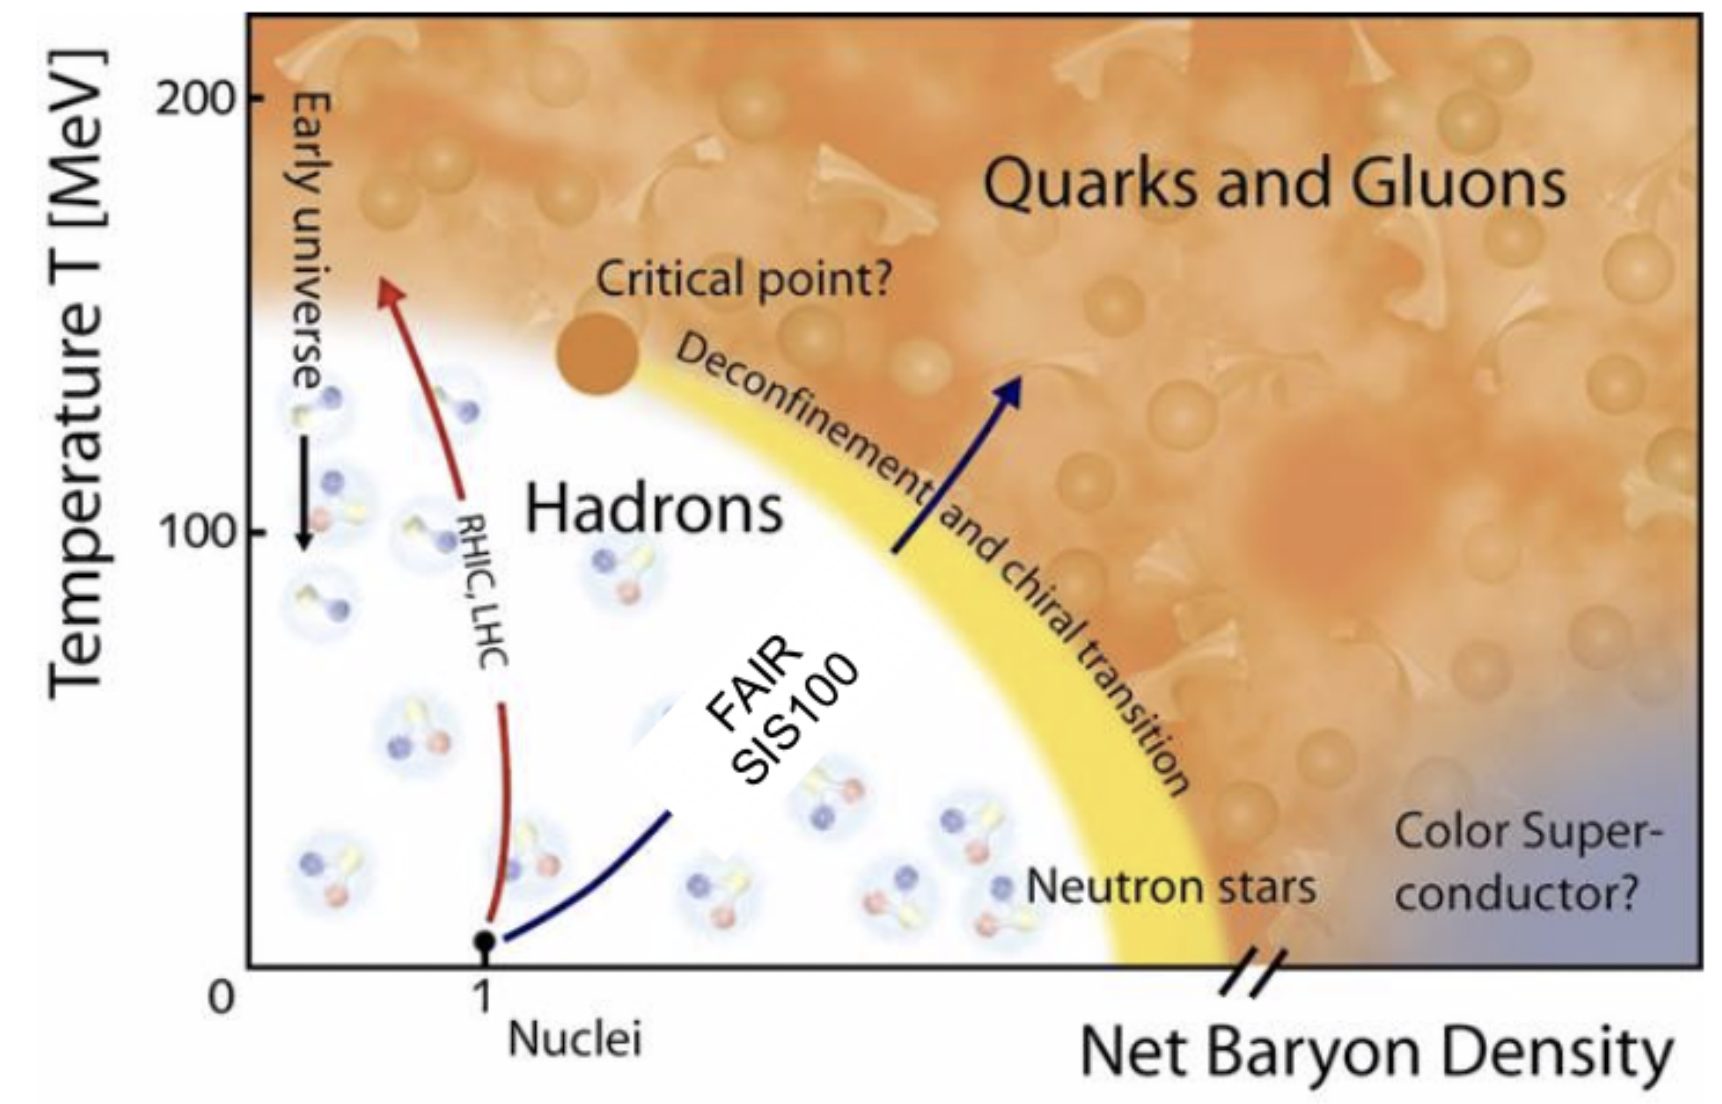
\includegraphics[width=.7\textwidth]{images/phase_diagram.png}
    \caption{Phase diagram of the QCD matter \cite{progress report}}
    \label{phase_diagram}
\end{figure}
%--------------- CBM SETUP
\subsection{CBM setup}
In order to identify the particles coming from the collisions, the setup of 8 detectors is under development in GSI Darmstadt\cite{progress report}.
\begin{figure}[H]
    \centering
    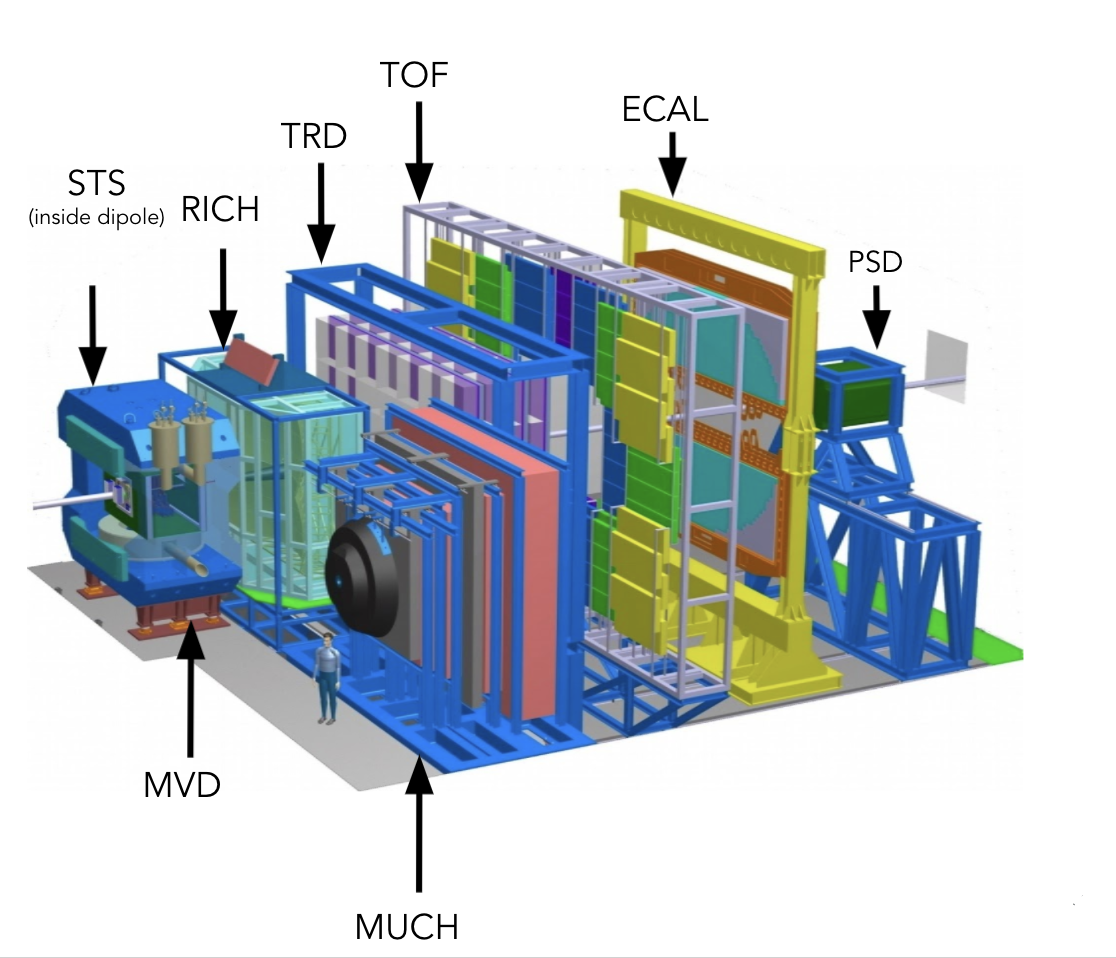
\includegraphics[width=.7\textwidth]{images/cbm_setup.png}
    \caption{CBM setup \cite{prezentacja gosi}}
    \label{cbm_setup}
\end{figure}
The CBM detectors setup will consist of:
\begin{itemize}
    \item STS - Silicon Tracking System
    \item MVD - Micro Vertex Detector
    \item RICH - Ring Imaging Cherenkov Detector, replaceable with:
    \item MUCH - Muon Chamber System
    \item TRD - Transition Radiation Detector
    \item TOF - Time of Flight Detecotor
    \item ECAL - Electromagnetic Caloromiter
    \item PSD - Projectile Spectator Detector
\end{itemize}
While each detector has its own role, in this work I will mainly focus on the results coming from two of them: charged particles like protons or pions can be identified using the Time of Flight Method\cite{tof}, which bases on the TOF detector; the short-lived particles reconstruction depends mainly on the STS detector.
%---------------- Physical motivation
\section{Physical motivation}
%---------------- Strange particles reconstruction
\subsection{Strange particles reconstruction}
In the nuclei collisions in experiments like CBM or HADES, the strange quarks are only produced during collisions. Thus, they provide information about the evolution of nuclear matter. We expect \cite{deconfinement} that in the \emph{mixed phase} (when both nucleon and quark degrees of freedom are present), which can be produced at FAIR energies, the yield of strange particles could be comparable with particles composed of \emph{u} and \emph{d} quarks. To verify this, we need to reconstruct all the strange particles, also short-lived strange particles like \PLambda$^0$, \PXiminus, \PKshort which cannot be detected directly.

\begin{figure}[H]
    \centering
    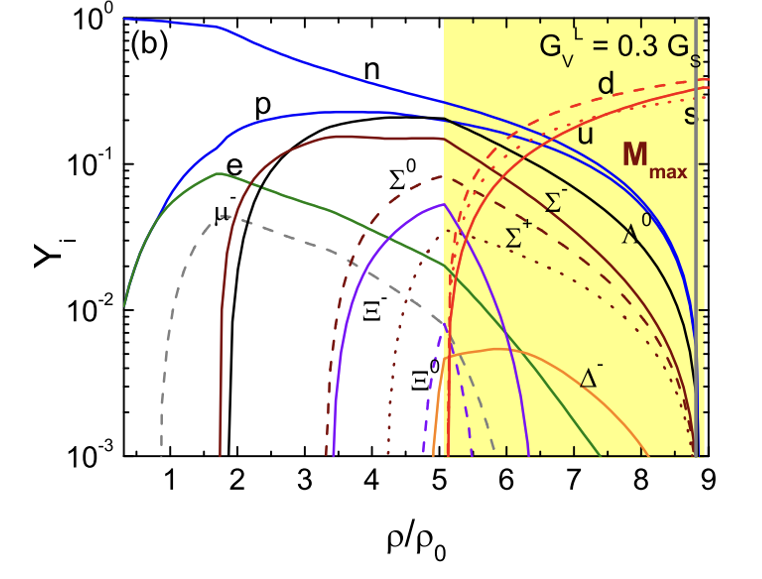
\includegraphics[width=.6\textwidth]{images/mixed_phase.png}
    \caption{Particle population vs density (mixed phase highlighted in yellow) \cite{deconfinement}}
    \label{cbm_setup}
\end{figure}
%------------- K-short reconstruction
\subsection{\PKshort reconstruction}
\noindent\begin{minipage}{0.6\textwidth}
In this work, I will mainly focus on the reconstruction of one of the short-lived particles, K-short (short-lived Kaon):
\begin{itemize}
    \item Mass: 497.611 \pm\ 0.013 MeV/$c^2$
    \item Mean lifetime: $8.958\cdot 10^{-11}$ s
    \item Charge = 0
    \item Meson, composed of two quarks: \Pdown\APstrange or \Pstrange\APdown
    \item Strange particle
    \item in the main decay mode (69.2\% of cases) decays into \Pgpp and \Pgpm \cite{kdecay2}
\end{itemize}
\end{minipage}
\noindent\begin{minipage}{0.4\textwidth}
    \centering
    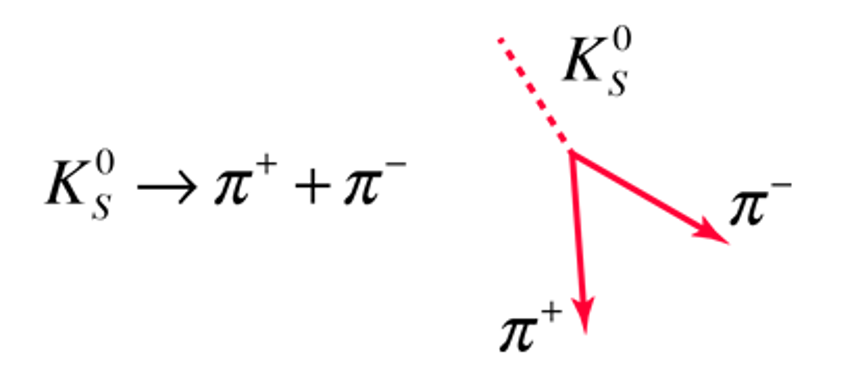
\includegraphics[width=\textwidth]{images/kdecay1.png}
    \PKshort main decay mode \cite{kdecay1}
\end{minipage}
The main decay mode of \PKshort is more symmetric than e.g., \PLambda$^0$ main decay mode (decay into \Pproton and \Pgpm); its products are also less massive than the ones coming from \PLambda$^0$ decay. Therefore, the investigation of this decay can tell us much about the tracking performance in CBM. Also, we can explore the influence of the magnetic field strength on the efficiency of the reconstruction of short-lived particles.

%---------------- short-lived particles reconstruction
\chapter{Short-lived particles reconstruction}
%------------------------ KFParticleFinder
\section{KFParticleFinder}
Short-lived particles like \PLambda$^0$, and \PKshort (mean lifetime respectively: $2.631 \cdot 10^{-10}$~s, and $8.958\cdot 10^{-11}$~s) have neutral charge, therefore they cannot be detected directly. However, we can reconstruct these particles by investigating their \emph{daughter particles}, particles coming from their decays. Using i.e. the Silicon Tracking System we can reconstruct the tracks of pions coming from \PKshort decay. In order to do so, the \emph{KFParticleFinder} was developed \cite{kfp}. It is an on-line optimized reconstruction package based on Kalman Filter mathematics. It finds pairs of positive and negative pions (in our case) which could be a result of K-short decay. 
%------------------------- PFSimple
\section{PFSimple}
For offline selection optimization and analysis, PFSimple package was created \cite{pfsimple}. Using it, one can optimize selection criteria to differentiate between:
\begin{itemize}
    \item signal - pion pairs created in K-short decay
    \item background - pions pairs returned by KFParticleFinder which are not the result of K-short decay
\end{itemize}
Also, PFSimple returns these attributes of each reconstructed particle:
\begin{itemize}
    \item L/$\Delta$L - distance between primary and secondary vertex divided over its error
    \item DCA - distance of closest approach between pion tracks
    \item $\chi^2$ geo - dimensionless distance of closest approach between pion tracks
    \item $\chi^2$ topo - dimensionless distance of closest approach between extrapolated kaon trajectory and primary vertex
    \item $\chi^2$ prim - dimensionless distance between extrapolated secondary track and primary vertex
    \item $\cos(\alpha)$ - cosine of angle between pion and K-short momenta
\end{itemize}
\begin{figure}[H]
    \centering
    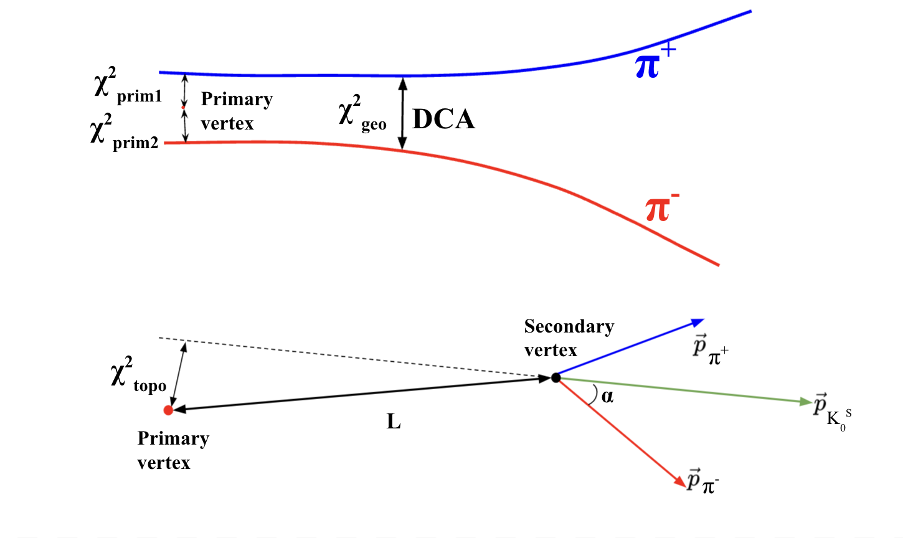
\includegraphics[width=.9\textwidth]{images/pfsimple_variables.png}
    \caption{Decay scheme and topological variables}
    \label{cbm_setup}
\end{figure}
%------------------------- optimization of selection criteria
\section{Optimization of selection criteria}
As the KFParticle Finder (and PFSimple) return the possible pion pairs, which could be a result of K-short decay,  some selection criteria need to be applied to differentiate between the signal and background.\\ Manual procedure for selection criteria optimization \cite{manual} is as follows:
\begin{itemize}
    \item The goal is to suppress as a lot background and to preserve as much signal as possible 
    \item Plot distribution of signal and background for some variable, and select a point above which all entries are considered as signal or background
    \item Repeat it for all the variables
\end{itemize}
\begin{figure}[H]
    \centering
    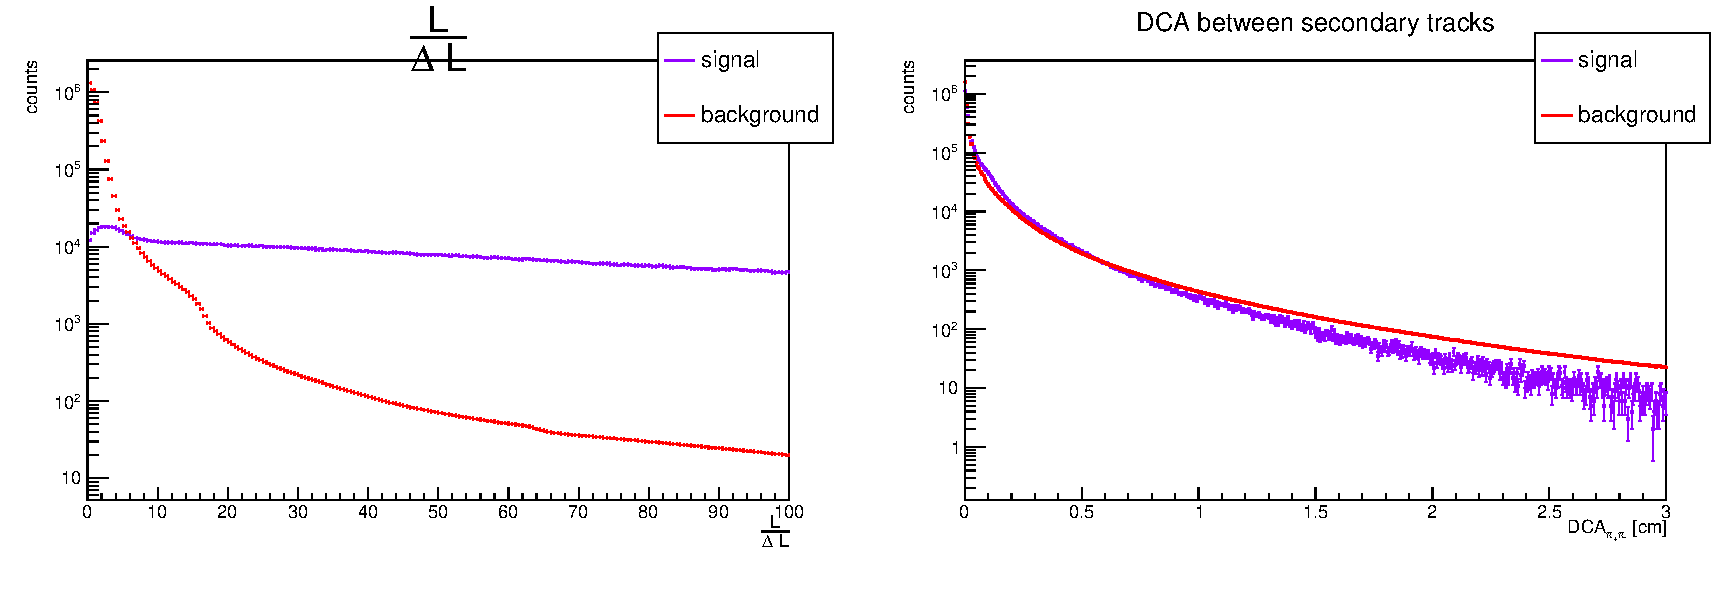
\includegraphics[width=1\textwidth]{images/pfsimple_distributions.pdf}
    \caption{Example of distributions to be checked with the manual selection criteria optimization}
\end{figure}

This method has the following advantages and drawbacks:
\begin{table}[h!]
    \begin{tabular}{l|l|}
    \hline
    \multicolumn{1}{|c|}{\textbf{Advantages}}  & \multicolumn{1}{c|}{\textbf{Disadvantages}}     \\ \hline
    \multicolumn{1}{|l|}{Easily interpretable} & Linear i.e. one dimension/variable is used once \\ \hline
    \multicolumn{1}{|l|}{Computationally inexpensive} & Non-automatized                                   \\ \hline
                                                      & Collision simulating model (e.g. UrQMD) dependent \\ \cline{2-2} 
    \end{tabular}
\caption{\label{tab:manualselection}Advantages and disadvantages of manual selection criteria optimization}
\end{table}

Another approach is using \emph{Machine Learning} to optimize selection criteria, which is the main topic of this work, and will be described in the next chapters.


%-------------------------- Machine Learning
\chapter{Machine Learning}
%------------------- supervised machine learning
\section{Supervised machine learning}
Supervised machine learning, is "a subcategory of machine learning and artificial intelligence. It is defined by its use of labeled datasets to train algorithms that classify data or predict outcomes accurately. As input data is fed into the model, it adjusts its weights until the model has been fitted appropriately, which occurs as part of the cross validation process."\cite{ibm}
%--------------- XGBoost
\section{XGBoost}
XGBoost  is a decision-tree-based (supervised) Machine Learning algorithm that uses gradient boosting. \cite{xgboost}. It is highly efficient when used with e.g., tabular data, so it suits the need for optimization selection criteria.\cite{shahid}
%--------- Decision trees
\subsection{Decision trees}
We can also visualize manual selection criteria with a decision tree:\\
1. For each variable of a reconstructed particle, a conditional statement is being set \\
2. If all conditions are fulfilled, a K-short candidate is treated as a signal  candidate\\
\begin{figure}[H]
    \centering
    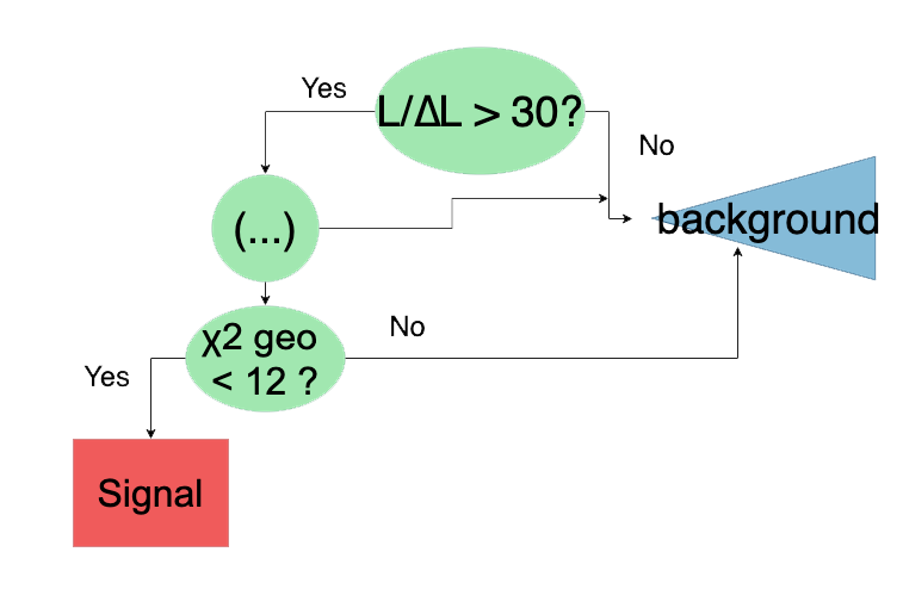
\includegraphics[width=.7\textwidth]{images/decision_tree.png}
    \caption{Example of a decision tree using manual selection criteria}
\end{figure}
In XGBoost, the algorithm creates multiple decision trees, combines them, and returns \textbf{\emph{probability}} whether a K-short candidate is a signal or background candidate.
\subsection{Comparison of ML with manual selection criteria }
\begin{table}[h!]
    \begin{tabular}{|l|l}
    \hline
    \multicolumn{1}{|c|}{\textbf{Advantages}}        & \multicolumn{1}{c|}{\textbf{Disadvantages}}    \\ \hline
    Non-linear in multi-dimensional space            & \multicolumn{1}{l|}{Not easily interpretable}  \\ \hline
    Automatization of the selection process          & \multicolumn{1}{l|}{Computationally expensive} \\ \hline
    Partially collision simulating model-independent &                                                \\ \cline{1-1}
    \begin{tabular}[c]{@{}l@{}}With \emph{probability} a  value from which we consider \\a particle as a K-short particle can be chosen;\\ it can aim for better reconstruction efficiency \\ or a better background reduction\end{tabular} &
       \\ \cline{1-1}
    \end{tabular}
\caption{\label{tab:mlselection}Advantages and disadvantages of ML selection criteria optimization}
\end{table}

%----------- Data preparation
\chapter{Data preparation}

%---------------- Data enriching
\section{Data enriching}
There are two problems to tackle before providing datasets to our ML model: underrepresentation and dependence of collision simulation model.
%---------------underrepresentation
\subsection{Underrepresentation}
As in the simulated data, less than 0.1\% of K-short candidates are signal candidates, the ratio in the training dataset has to be changed so that the model learns how to identify signal candidates well. The number of background entries is rescaled by this formula:
\begin{equation}
    n_\text{events(background)} = 5 \cdot n_\text{events(signal)}
\end{equation}
\begin{figure}[H]
    \centering
    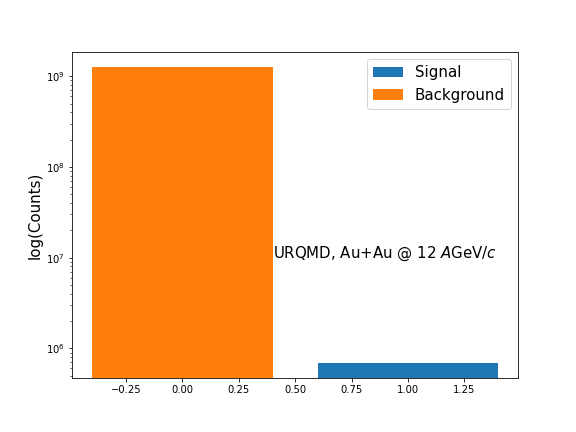
\includegraphics[width=.6\textwidth]{images/inbalance.png}
    \caption{Imbalance of classes}
\end{figure}
%---------------dependence of collision simulation model
\subsection{Dependence of collision simulation model}
To make the ML model partially independent of the collision simulation model,  select:
\begin{itemize}
    \item primary Ks candidates only in 5$\sigma$ region: $0.43485 - 0.56135$ (GeV/$c^2$) from DCM-QGSM-SMM model\cite{dcm}\cite{dcm2}, (simulation data)
    \item background outside 5$\sigma$ region from UrQMD model\cite{urqmd}, which mimics experimental data (will be replaced by real experimental data while CBM experiment starts)
\end{itemize}
Also, the UrQMD model is being used as a test dataset (as the model does not "know" the signal candidates from this MC model).
\begin{figure}[H]
    \centering
    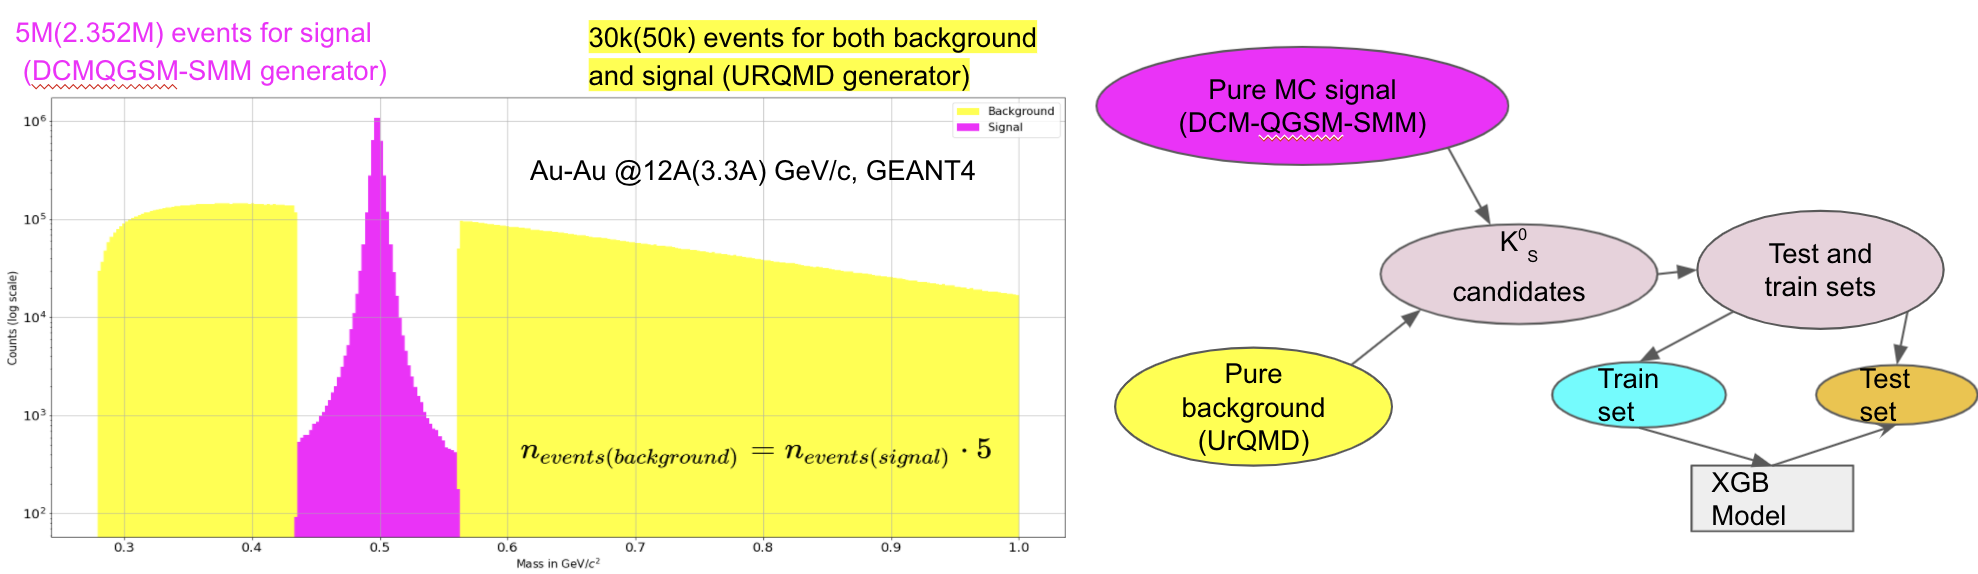
\includegraphics[width=1\textwidth]{images/dataset.png}
    \caption{Data enriching}
\end{figure}
In total, the following datasets will be used:
\begin{itemize}
    \item 5M (2.352M) events for signal generated in DCM-QGSM-SMM
    \item 30k(50k) events for both background and test dataset generated in UrQMD
\end{itemize}
Au-Au @12A(3.3A) GeV/c passed through CBM setup in GEANT4.\cite{geant4}\cite{geant4 2}
%------------- data cleaning
\section{Data cleaning}
To reject the numeric values of parameters which do not have physical sense, but are present in the data set, some selection criteria are applied before the beginning of the model training. Similarly, we some values which might be possible but are rare enough are rejected, to reduce the amount of data.

%----------------------- Invariant mass
\subsection{Invariant mass}
As the K-short particle decays into two pions, its invariant mass cannot be smaller than the mass of the two pions, so:
\begin{center}
    $m_\text{inv} >$ 0.279 GeV/$c^2$
\end{center}
Also, to reduce the amount of data:
\begin{center}
   $m_\text{inv} <$ 1 GeV/$c^2$
\end{center}

%---------------- distances
\subsection{Distances and \emph{x, y, z} coordinates}
Distance between the primary vertex (the point where the collision of the nuclei happens), and the secondary vertex (the extrapolated point where the two daughter particles should have crossed each other)  - $l$ and the distance of closest approach between the two pions - $DCA$ - should not be smaller than zero:
\begin{center}
    $DCA$, $l$, $\frac{l}{\Delta l}$ $> 0$
\end{center}

Also, due to the sizes of the tracking system (the largest station has an area of 1m$^2$):
\begin{center}
    $DCA < 100 $ cm
\end{center}
For the same reason:
\begin{center}
    $|x|, |y| < 50$ cm
\end{center}
As the particle has to hit 3 stations of the tracking system, and the last two are placed above 80 cm:
\begin{center}
    $l < 80$cm
\end{center}
For the same reason, and because of the fixed target geometry of the detector:
\begin{center}
    $-1$ cm $< z < 80$ cm
\end{center}
To reduce the data, we set:
\begin{center}
    $\frac{l}{\Delta l} < 15000$
\end{center}
However, in the KFParticle package $l$ is assumed to be signed by design, and one can notice that actually, some data entries have a negative value of distance, for both signal and background. As the \emph{quality cuts} should be rather conservative, the following ranges are set:
\begin{center}
     $l >$ -5 (cm)\\
     $\frac{l}{\Delta l} >$ -25
\end{center}
%----------------- momentums
\subsection{Momentums}
The fixed target geometry of the detector requires that:
\begin{center}
    $p_Z > 0 $ GeV/c
\end{center}
To reduce the data:
\begin{center}
    $p < 20$ GeV/c; $p_T < 3$ GeV/c
\end{center}


%-------------- chi square
\subsection{Chi square}
Since $\chi^2$ is a squared distance, all the values must be larger than zero:
\begin{center}
    $\chi^2 > 0$
\end{center}
To reduce the data, following the maximal values are selected:
\begin{itemize}
    \item $\chi^2$ first and second $< 3 \cdot 10^7$
    \item $\chi^2_{geo} < 10000$
    \item $\chi^2_{topo} < 100000$
\end{itemize}



%----------------------- pseudorapidity
\subsection{Pseudorapidity}
As pseudorapidity depends on polar angle as $\eta = -\ln{\tan(\frac{\theta}{2})}$, and the Silicon Tracking System (STS) covers the polar angles between 2.5$^{\circ}$ and 25$^{\circ}$, for which the pseudorapidity values would equal:
\begin{center}
    $ 1.5< \eta < 3.82 $
\end{center}
However, due to the magnetic field, the pseudorapidity is constrained to following values:
\begin{center}
    $ 1.0< \eta < 6.5 $
\end{center}
with which we loose 0.06\% of data for signal (instead of 5.66\%) and 0.08\% of data for background (instead of 6.75\%)

%------------------ variables selection
\section{Variables selection}
The last step before training our model is the selection of variables which will be used in the training of the discriminator. To make the model simpler, there is no need to use two variables if they are strongly correlated with each other. Also, to avoid signal/background classification directly by invariant mass, variables strongly correlated with the invariant mass of background should be omitted.
\subsection{Correlation matrix}
The Pearson correlation efficient is being calculated following this formula:
\begin{equation}
    \rho = \frac{\operatorname{COV}(X, Y)}{\sigma_X \times \sigma_Y}
\end{equation}
where $\operatorname{COV(X, Y)} = \operatorname{E}\left[\left(X - \operatorname{E}\left[X\right]\right) \left(Y - \operatorname{E}\left[Y\right]\right)\right]$; $\sigma_X = \sqrt{\operatorname{E}\left[\left(X - \operatorname{E}\left[X\right]\right)^2\right]}$
of each variable and plot it in a matrix:

\begin{figure}[H]
    \centering
    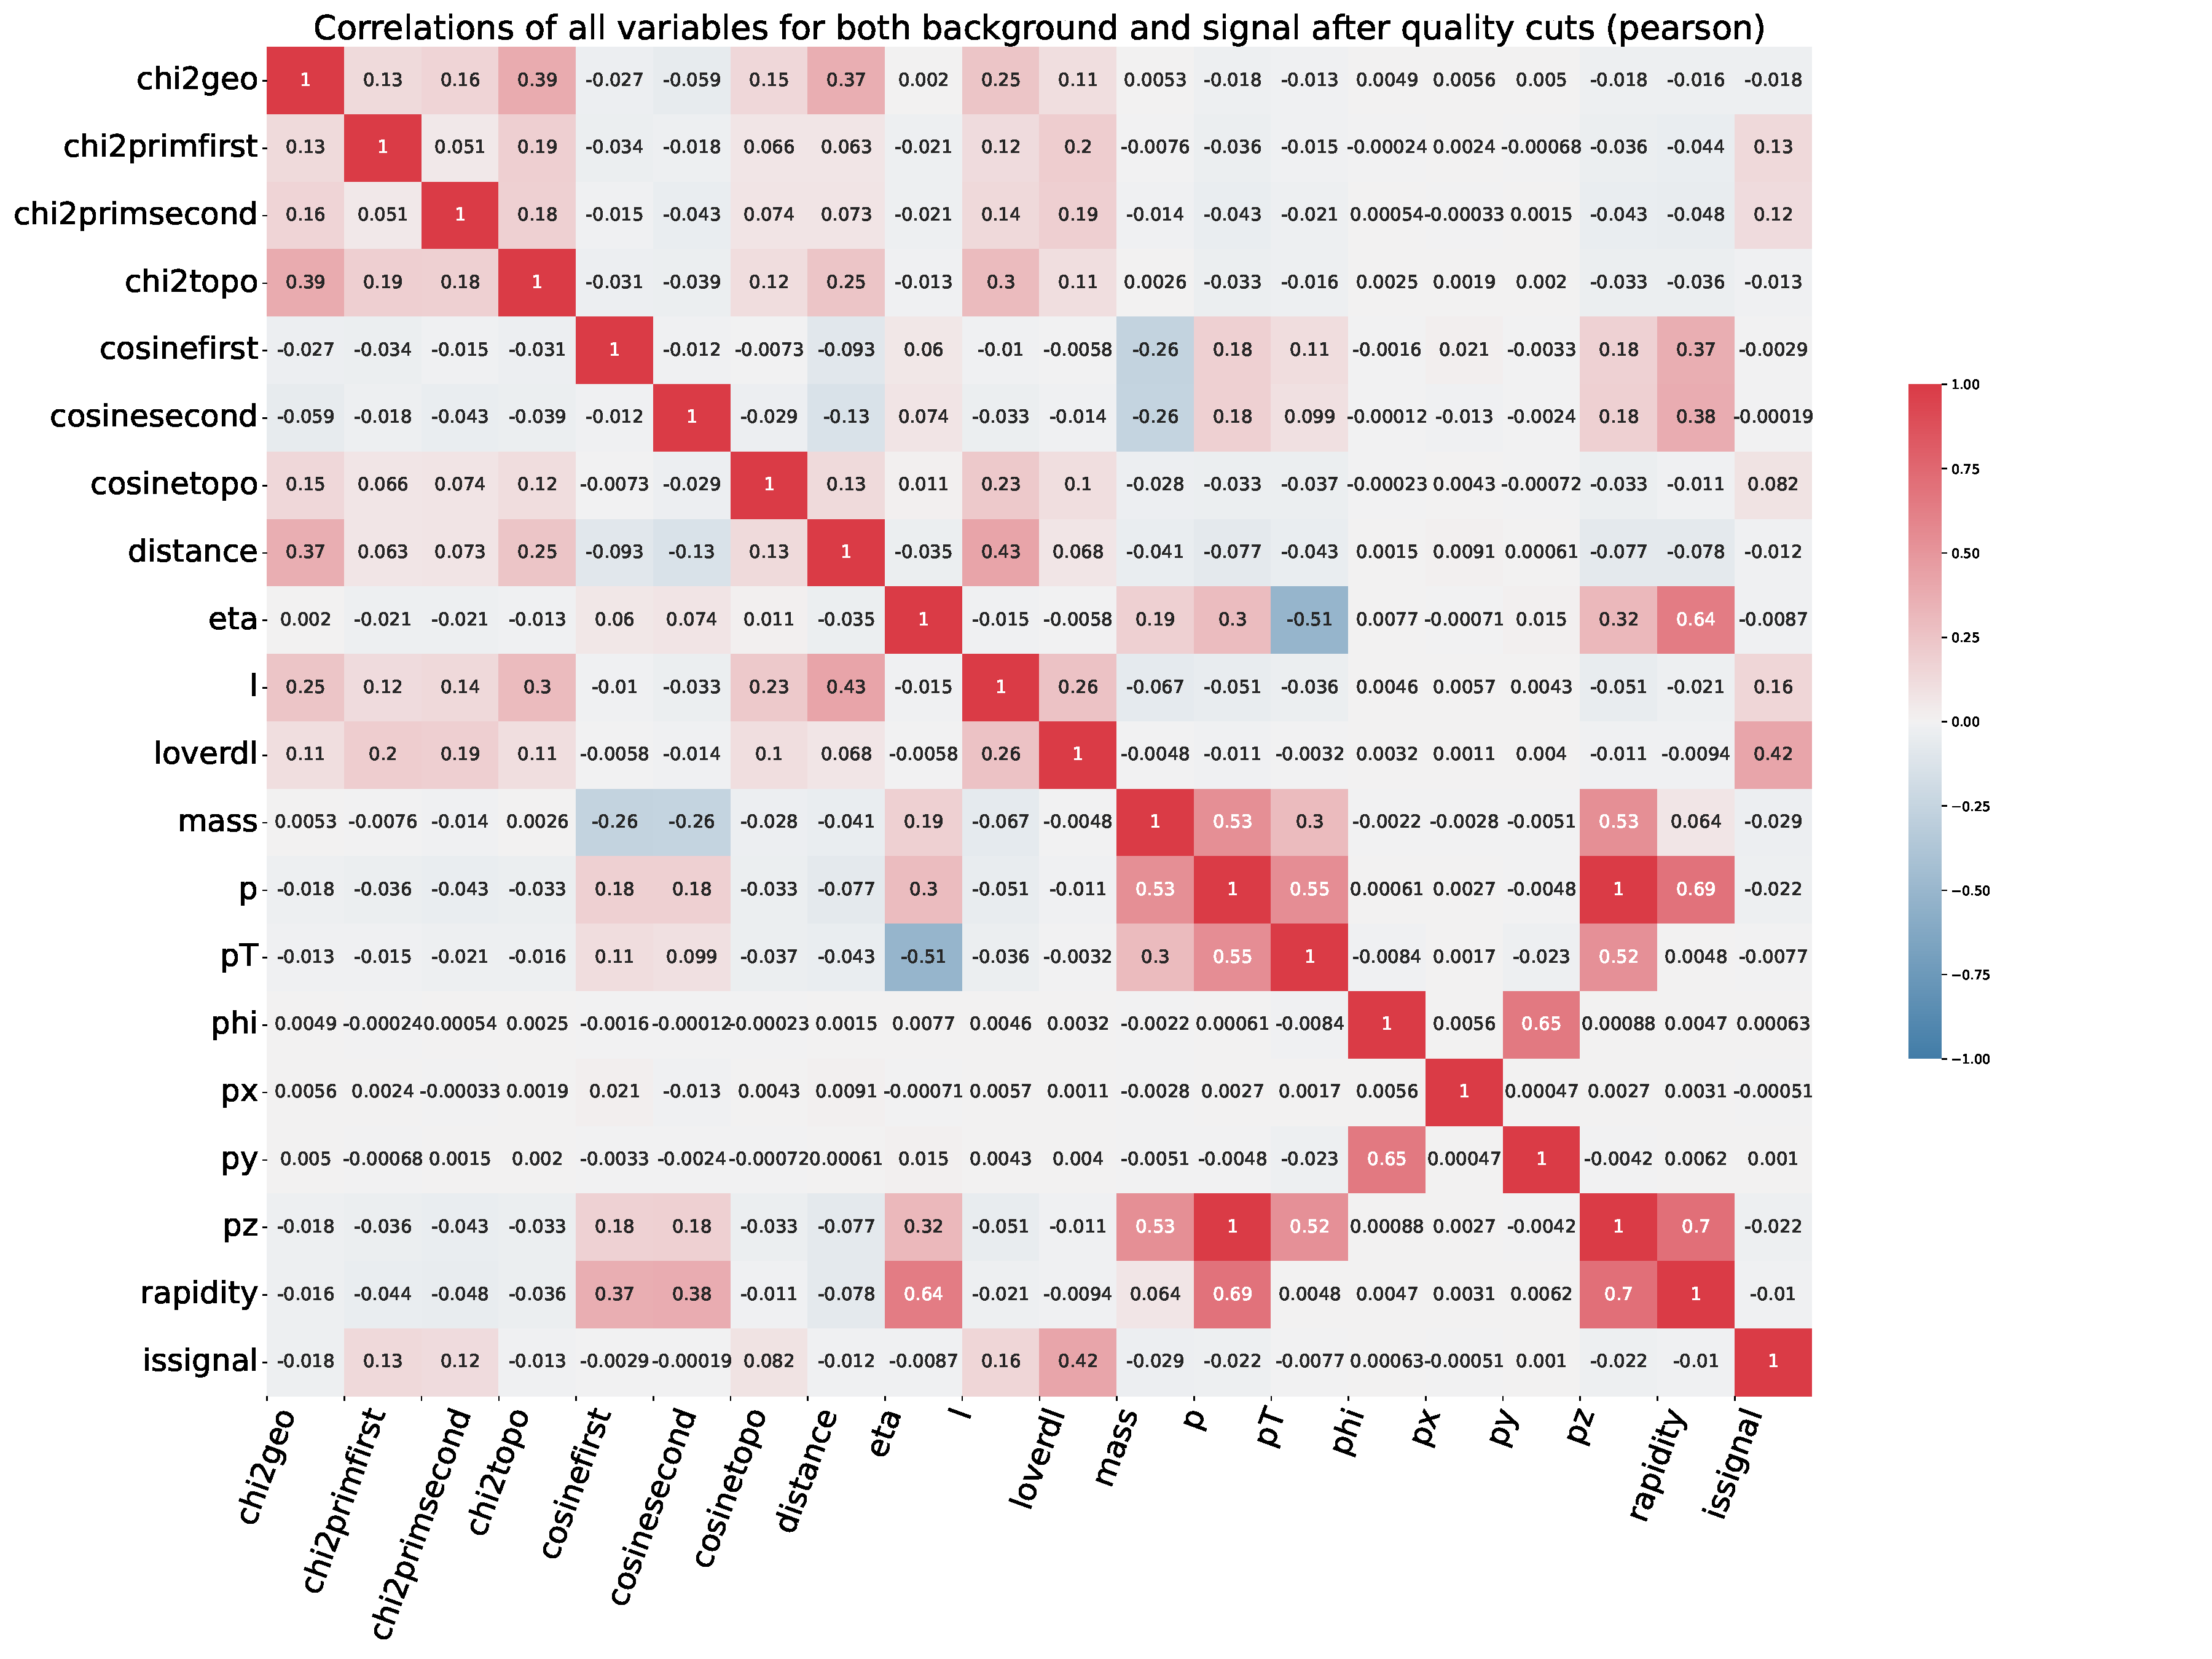
\includegraphics[width=1.2\textwidth]{images/Correlations_of_all_variables_for_both_background_and_signal_after_quality_cuts_(pearson).pdf}
    \caption{Correlation matrix}
\end{figure}
%-------------------- Correlation with invariant mass
\subsection{Correlation with invariant mass}
Later, the correlation (Pearson coefficient) of each variable with the invariant mass of (separately) signal and background is being checked 
\begin{figure}[H]
    \centering
    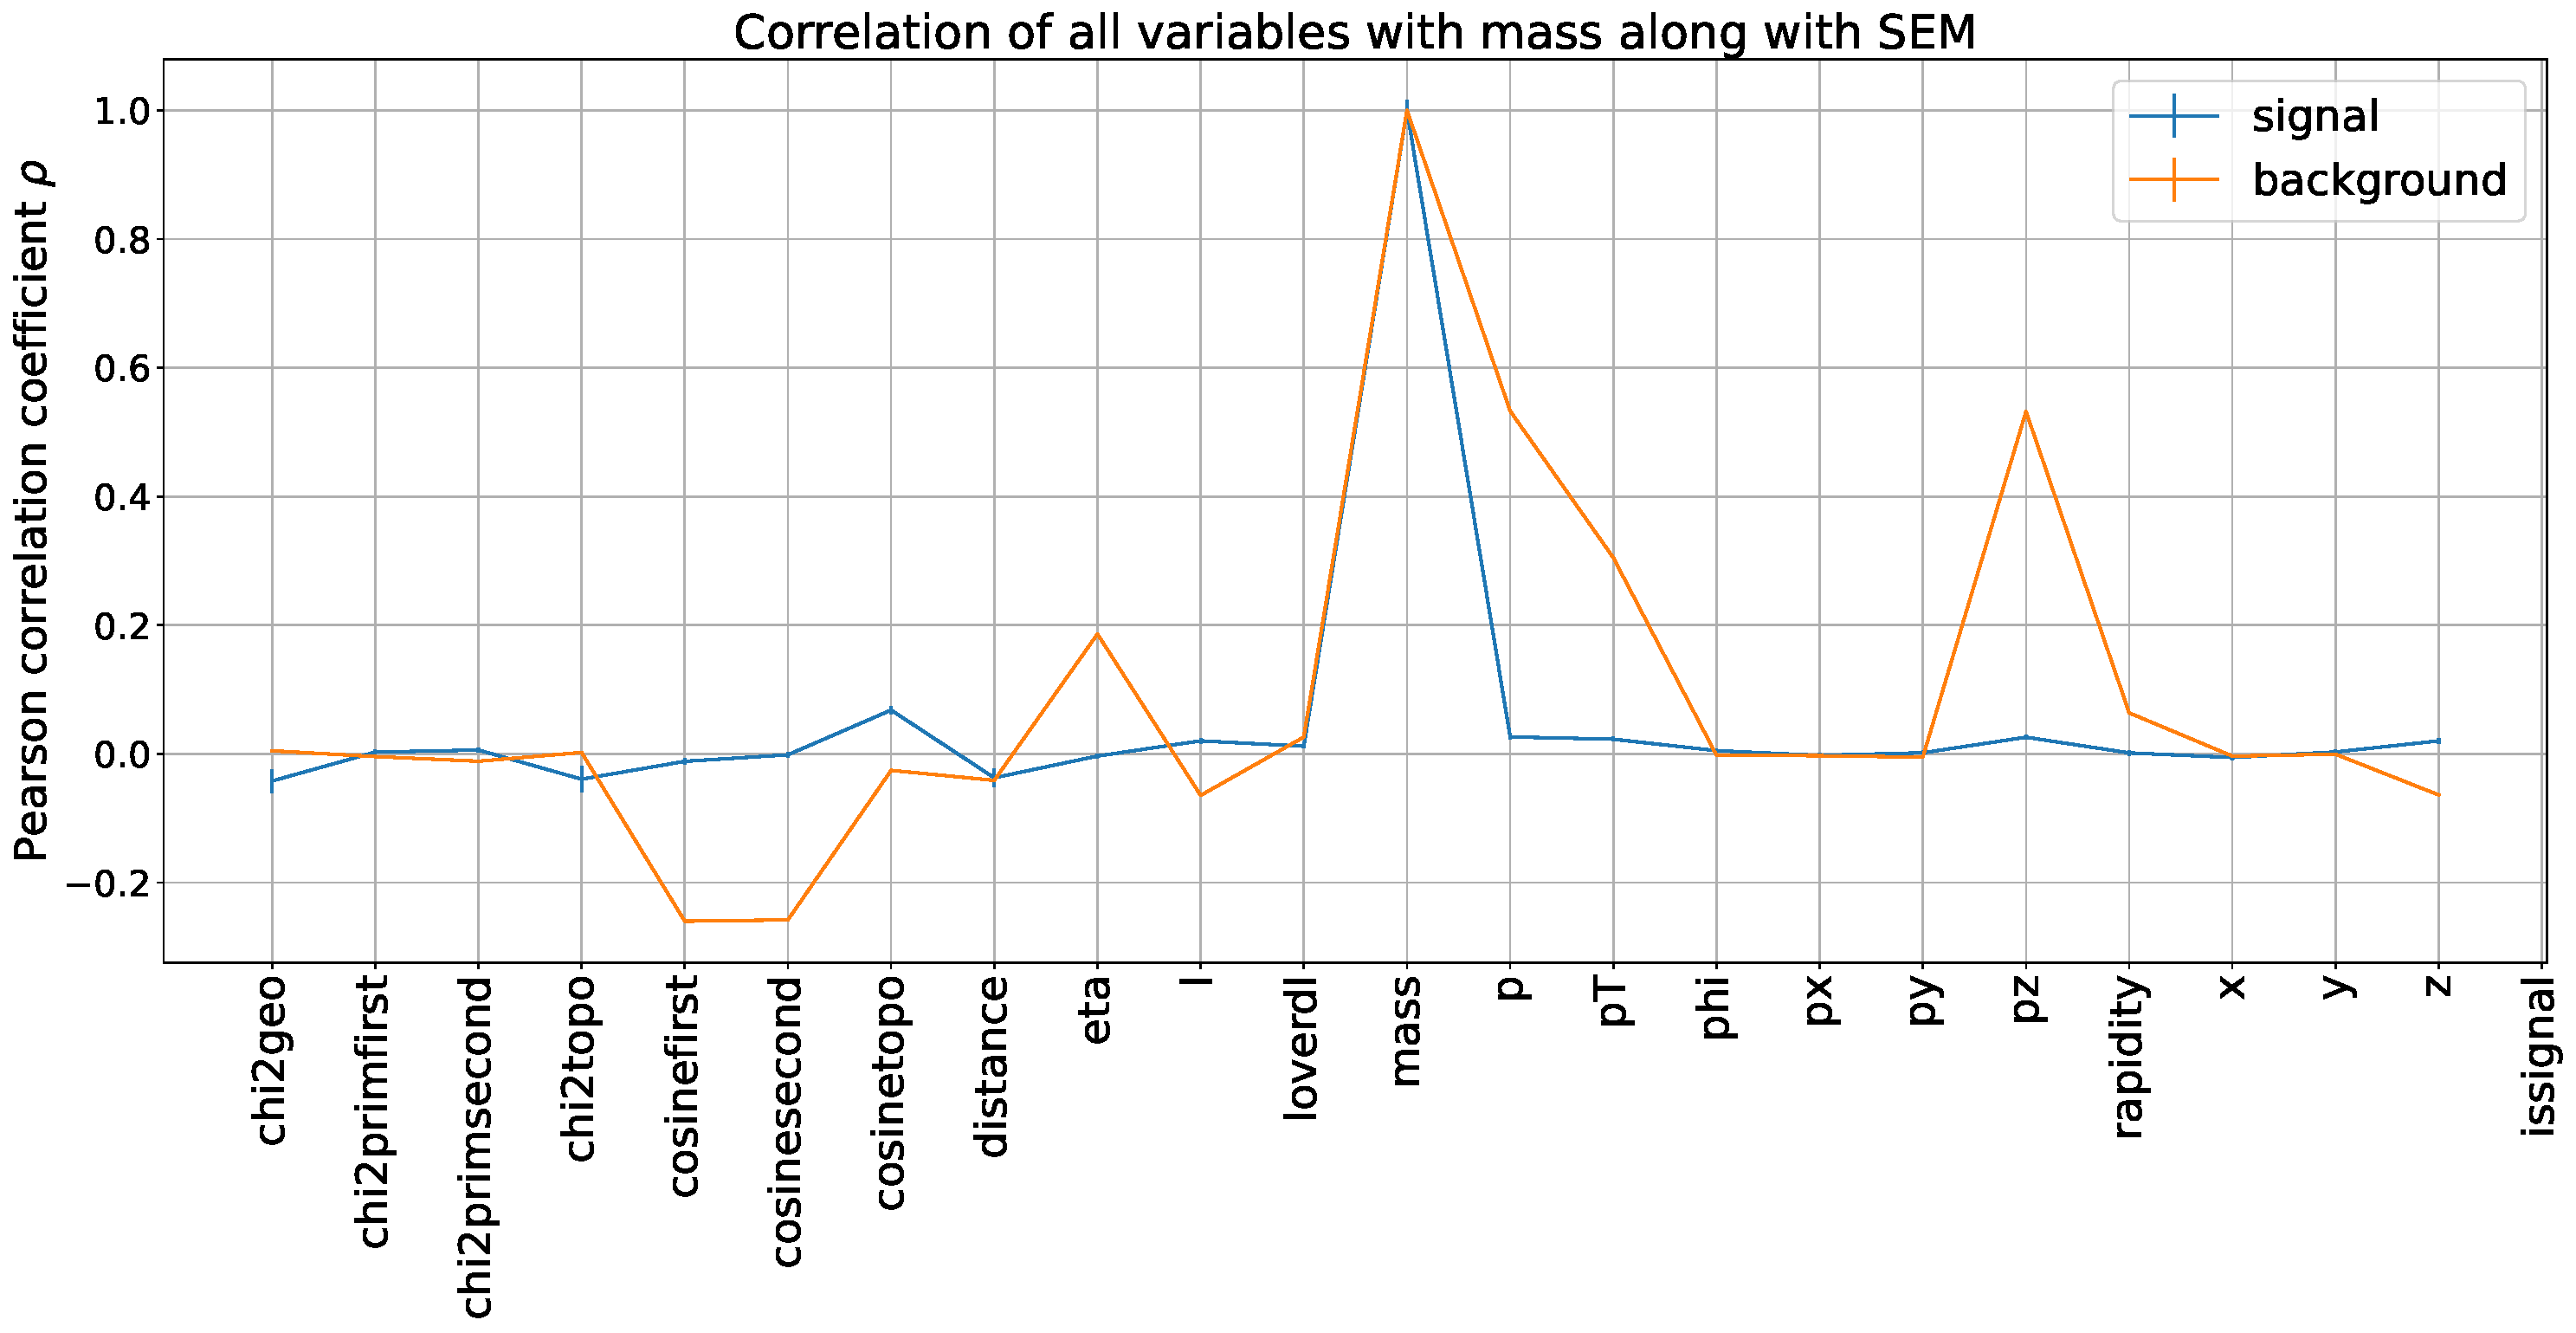
\includegraphics[width=1\textwidth]{images/Correlation_of_all_variables_with_mass_along_with_SEM.pdf}
    \caption{Correlation of all variables with mass}
\end{figure}
Also, a study of non-linear correlations has been performed. \cite{non-linear}

%-------------------- Selected variables
\subsection{Selected variables}
Based on that, the following 6 variables are selected for the training: $L/\Delta L$, $DCA$;  $\chi^2_{geo}$, $\chi^2_{topo}$, $\chi^2_{prim first}$, $\chi^2_{prim second}$

%----------------------- Model training
\chapter{Model training}
%--------- results for 12A GeV/c
\section{Results for $p_{\text{beam}}$ = 12A GeV/c}
Having prepared the data, the training of the ML algorithm may be initiated. To choose the hyper-parameters of the XGBoost model, the Bayesian Optimisation package was used.\cite{bayesian}\\
%--------------- Cross validation
\subsection{Cross validation}
To check if the model works as well on new data, as on the training dataset,  Receiver Operating Characteristic and probability plot are prepared.

\subsubsection{Receiver Operating Characteristic}
Receiver Operating Characteristic illustrates the diagnostic ability of a binary classifier. Threshold on the ROC (Receiver Operating Characteristic) curve which maximizes Approximate Median Significance 
\begin{equation}
    \text{AMS}= \sqrt{2} [(tpr + fpr) \log(1 + tpr/fpr) - tpr]
\end{equation}
(where $t(f)pr$ is true (false) positive rate) on the test sample is the best threshold.
\begin{figure}[H]
    \centering
    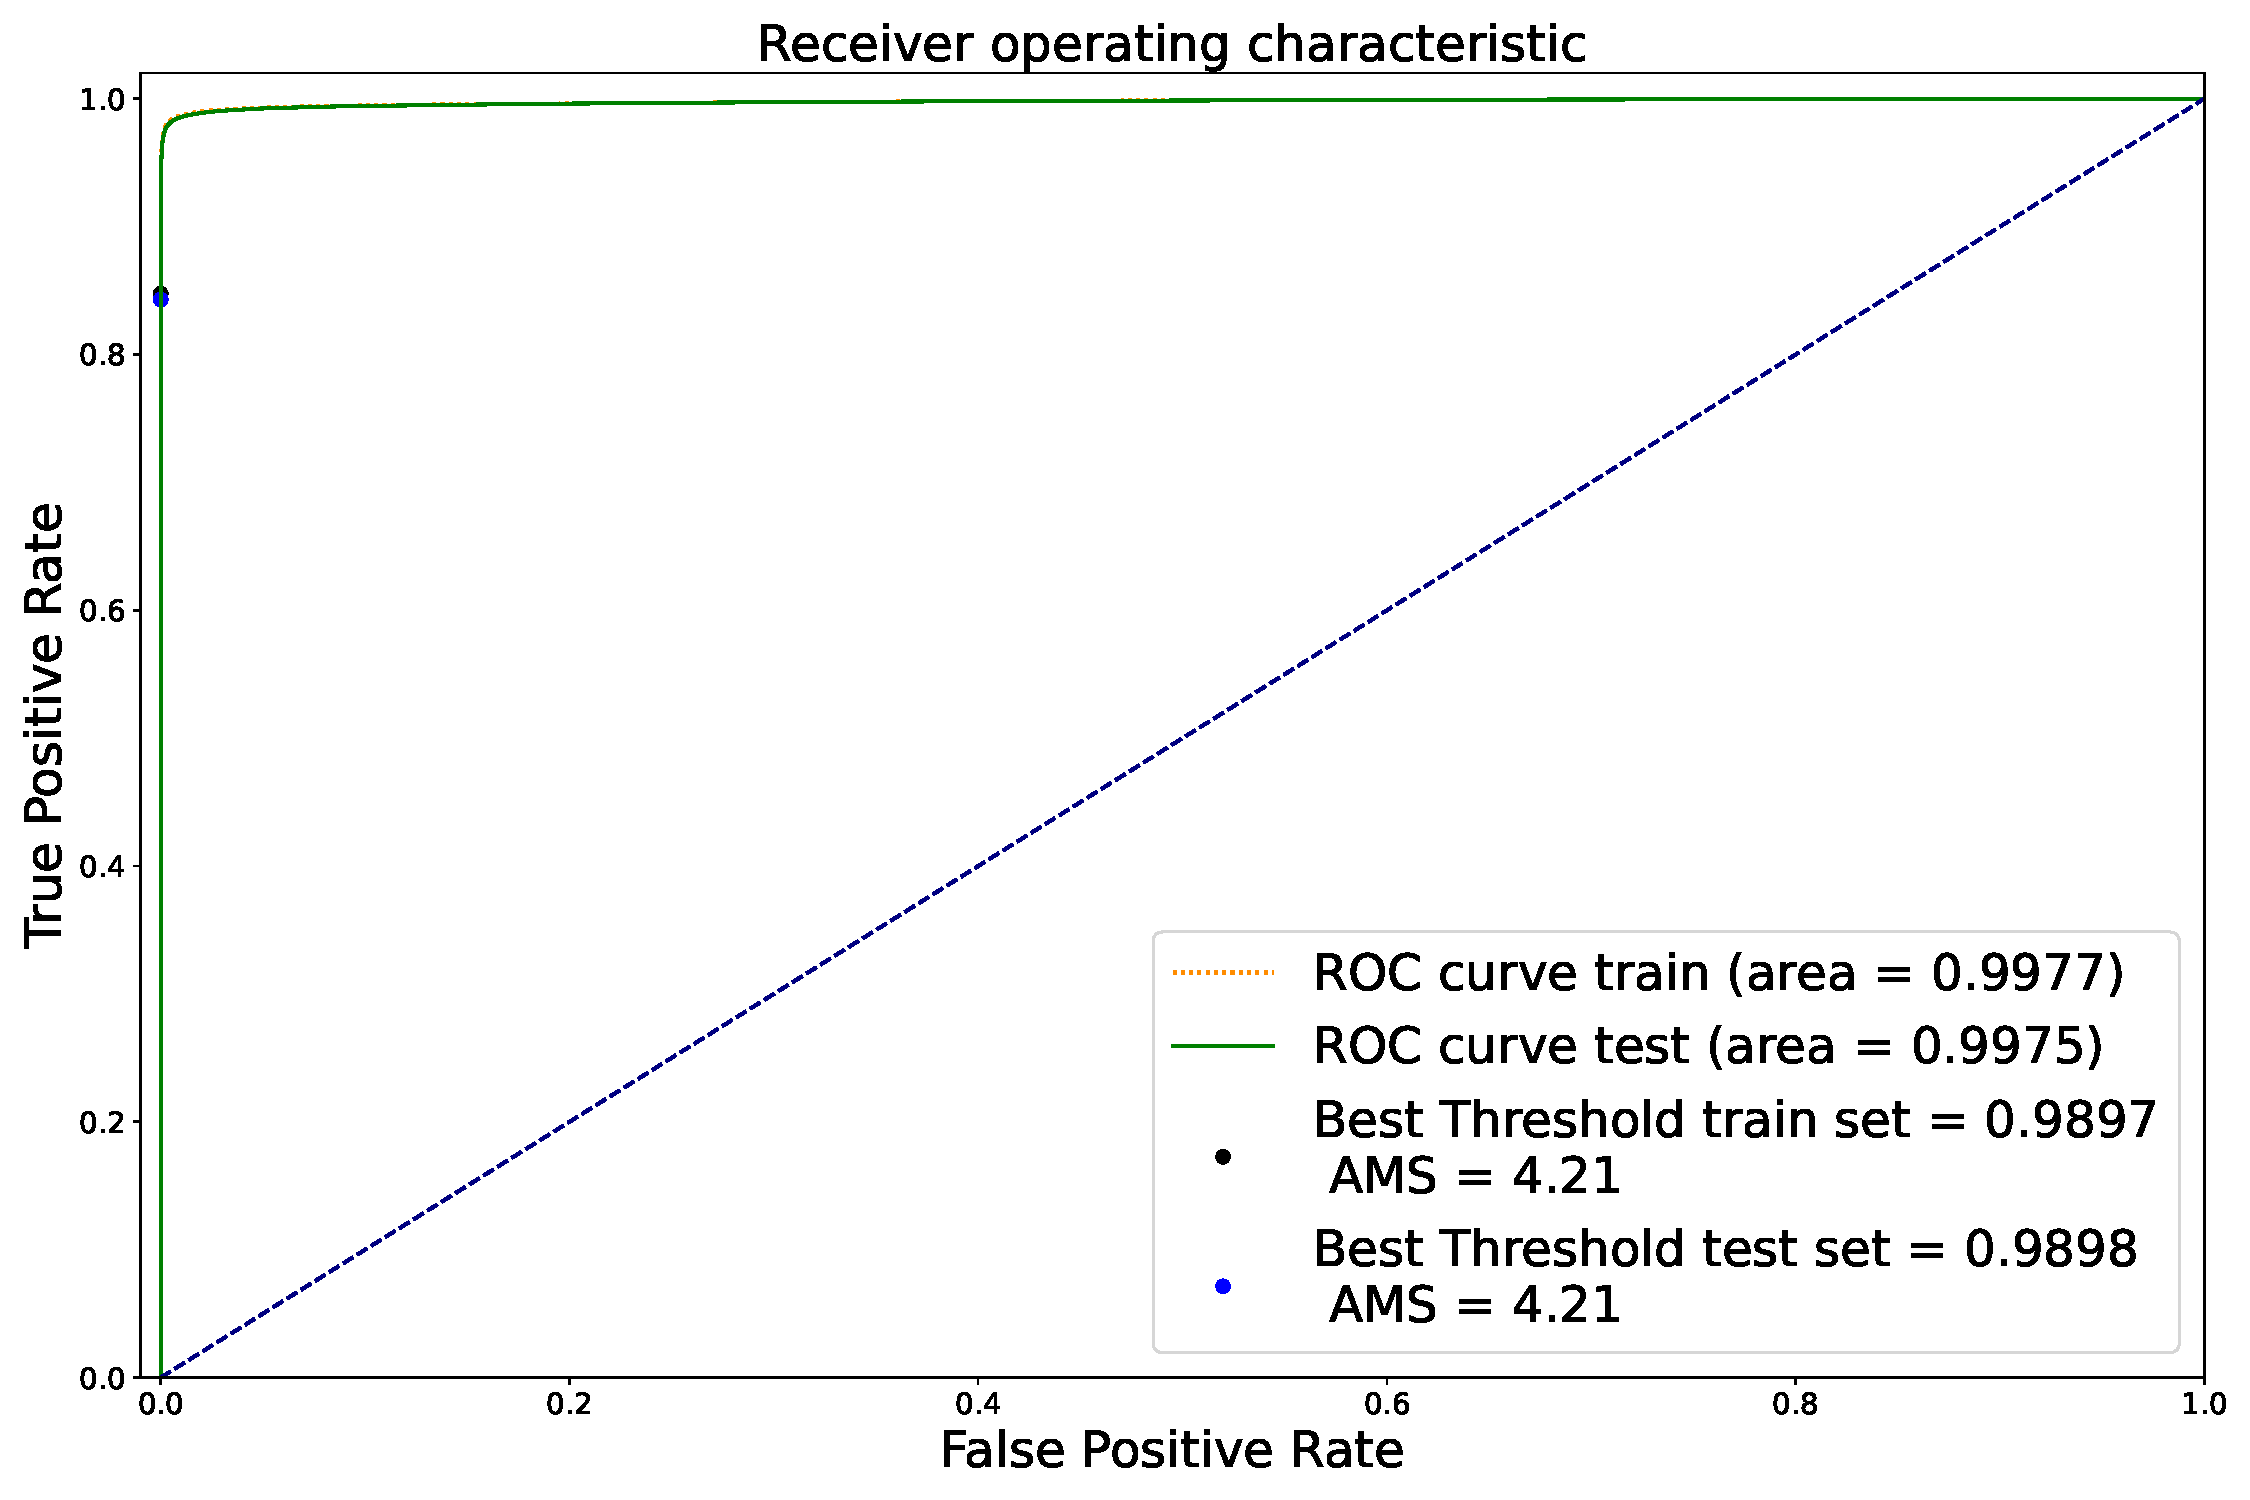
\includegraphics[width=1\textwidth]{images/ams.pdf}
    \caption{Receiver Operating Characteristic}
\end{figure}
We see that the optimal point on ROC is similar for both train and test datasets.
\subsubsection{Probability plot}
The graph of signal/background share in both train and test datasets is also plotted.
\begin{figure}[H]
    \centering
    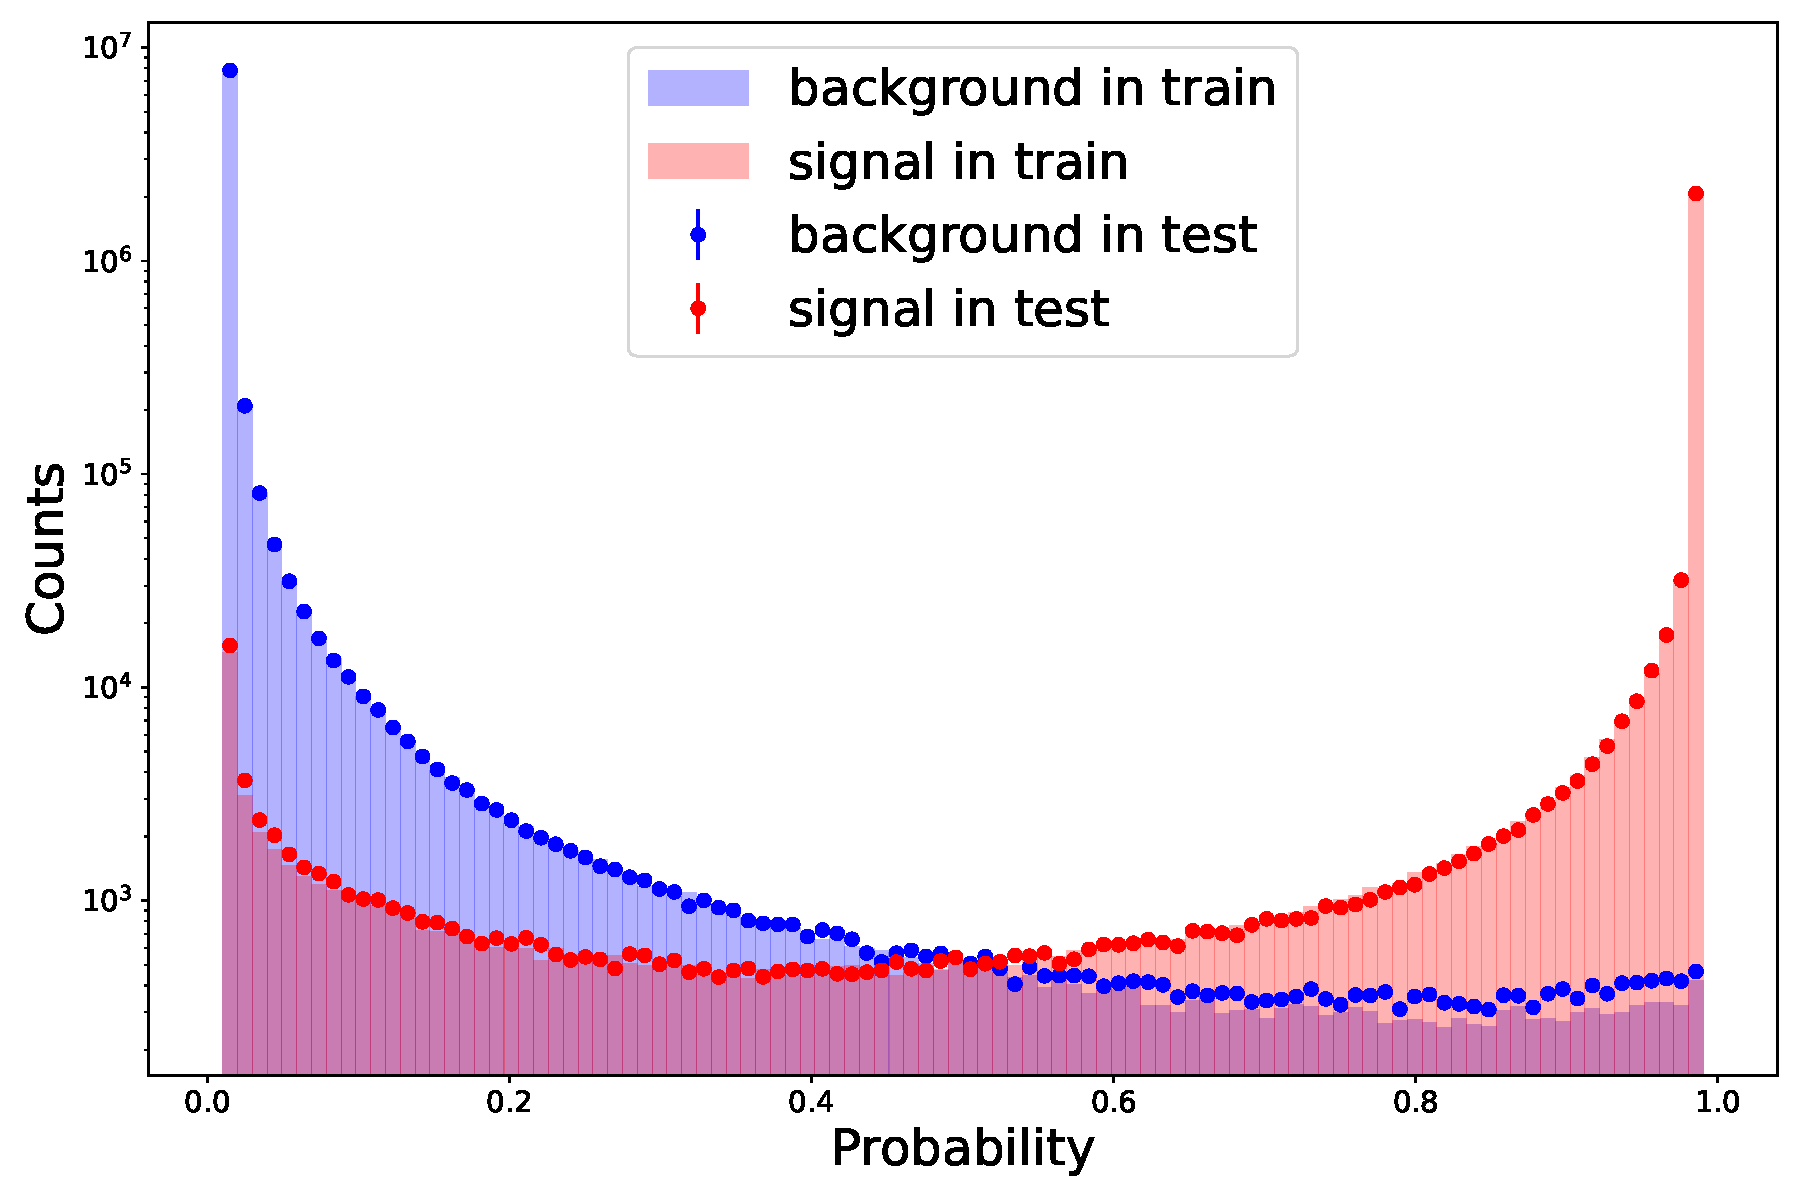
\includegraphics[width=.8\textwidth]{images/probability.pdf}
    \caption{Probability plot}
\end{figure}

Once again, the results are similar for the two datasets. Hence, we can say that our model is not overtrained (works well on new data).

\subsubsection{Invariant mass distribution}
\begin{figure}[H]
    \centering
    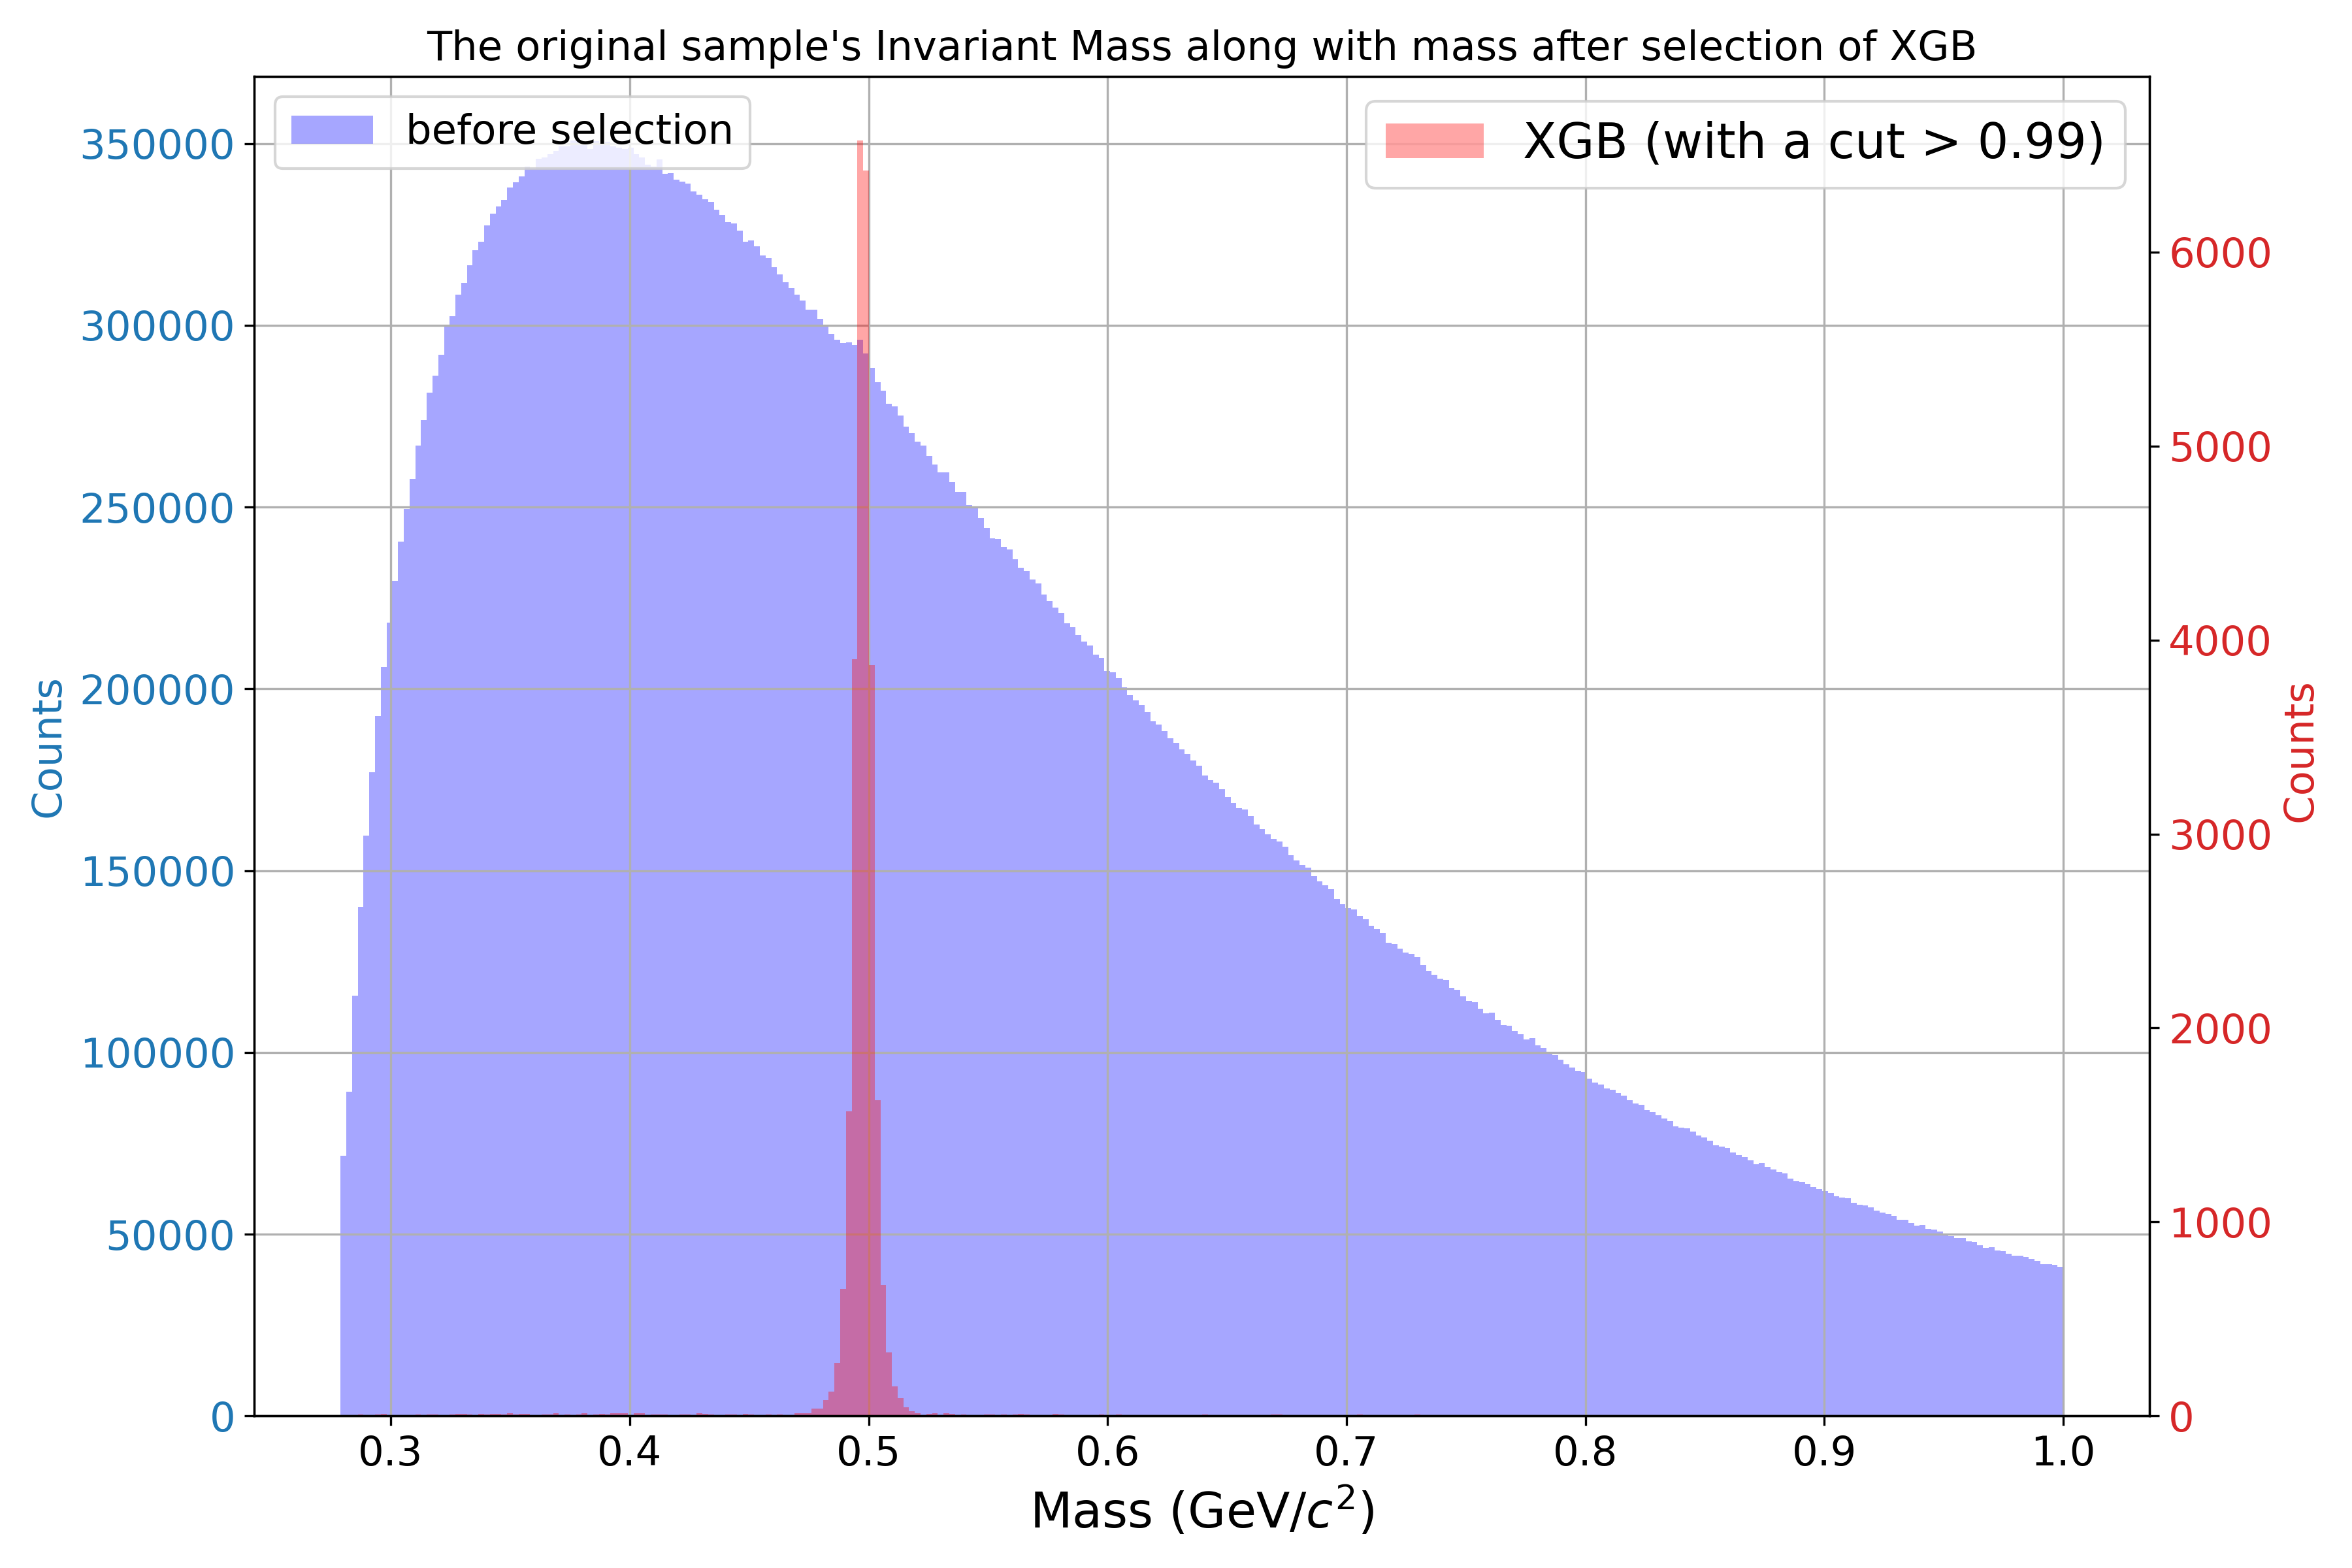
\includegraphics[width=.9\textwidth]{images/cut_visualization.png}
    \caption{Invariant mass distribution}
\end{figure}


%--------------- Comparison with default KFPF Cuts
\subsection{Comparison with default KFPF Cuts}
KFParticleFinder has default selection criteria, which can be compared with ML selection:
\begin{itemize}
    \item $L/\Delta L > 5 $
    \item $DCA < 1 $ cm
    \item $\chi^2_{geo} < 3 $
    \item $\chi^2_{prim} > 18.4 $
    \item $\cos(\alpha) > 0 $
\end{itemize}
Depending on the cut value,  better background reduction or better efficiency can be obtained.

\subsubsection{Better background reduction}
With a cut value set to 0.99, we get $50\times$ less background (Fig. \ref{bckgr}):
\begin{itemize}
    \item \textbf{Reconstructed \PKshort / reconstructible \PKshort = 80.67\%}  vs. 76.93\% with default KFPF cuts
    \item \textbf{false / true positive rate = 0.04} vs. 2.01 with default KFPF cuts
\end{itemize}
\begin{figure}
 \centering
    \begin{subfigure}[b]{0.99\linewidth} 
        \centering
        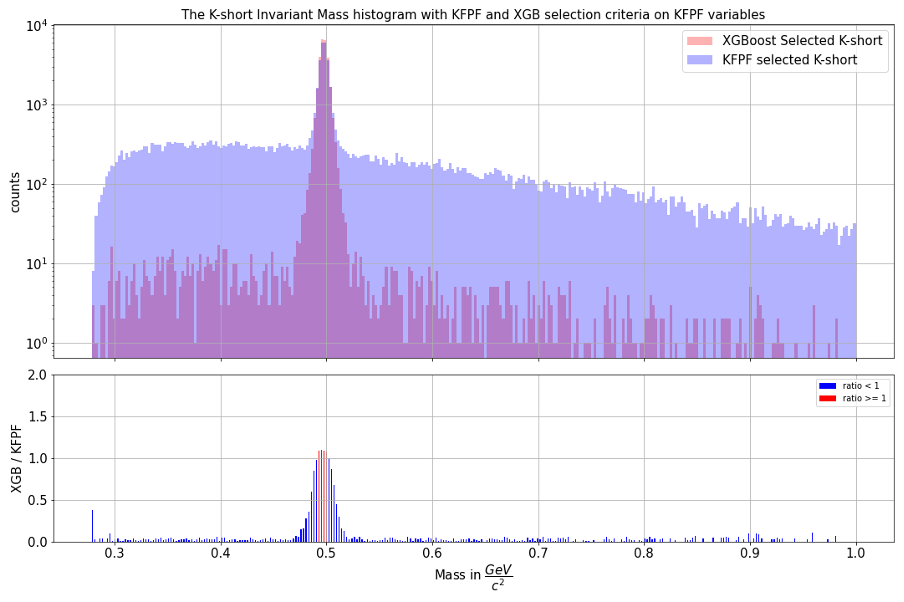
\includegraphics[width=\textwidth]{images/better_reduction1.png} 
        \caption{Invariant mass distribution (y log scale)} 
        \vspace{0.3cm}
    \end{subfigure}
     \hfill
       \begin{subfigure}[b]{0.99\linewidth}
        \centering
        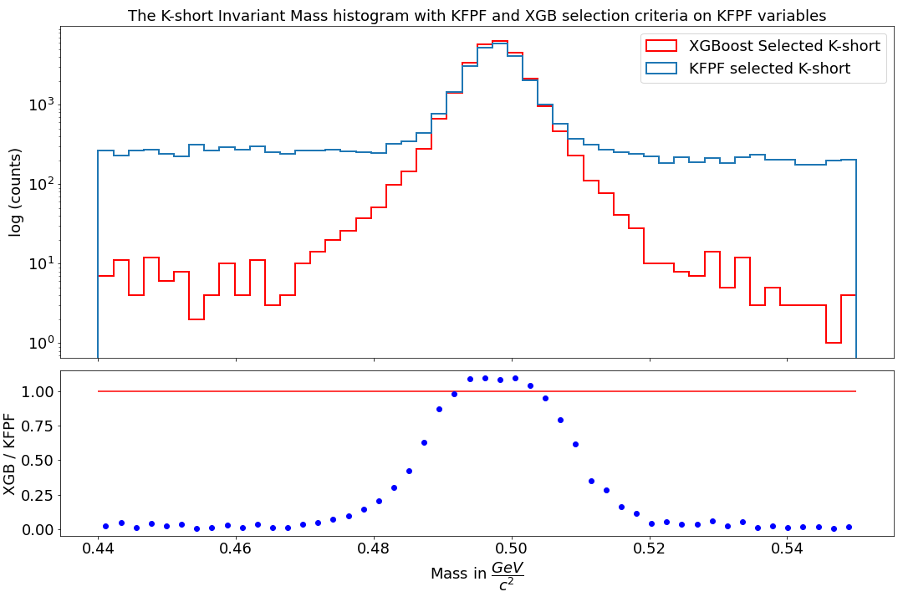
\includegraphics[width=\textwidth]{images/better_reduction2.png} 
        \caption{Invariant mass distribution (close-up)}
        \vspace{0.3cm}
    \end{subfigure}
    \caption{Comparison with KFPF cuts}\label{bckgr}
\end{figure}

\subsubsection{Better efficiency}
With a cut value set to 0.86, we get $20\%$ better efficiency (Fig. \ref{effic}):
\begin{itemize}
    \item \textbf{Reconstructed \PKshort / reconstructible \PKshort = 95.91\%}  vs. 76.93\% with default KFPF cuts
    \item \textbf{false / true positive rate = 1.27} vs. 2.01 with default KFPF cuts
\end{itemize}
\begin{figure}
 \centering
    \begin{subfigure}[b]{0.99\linewidth} 
        \centering
        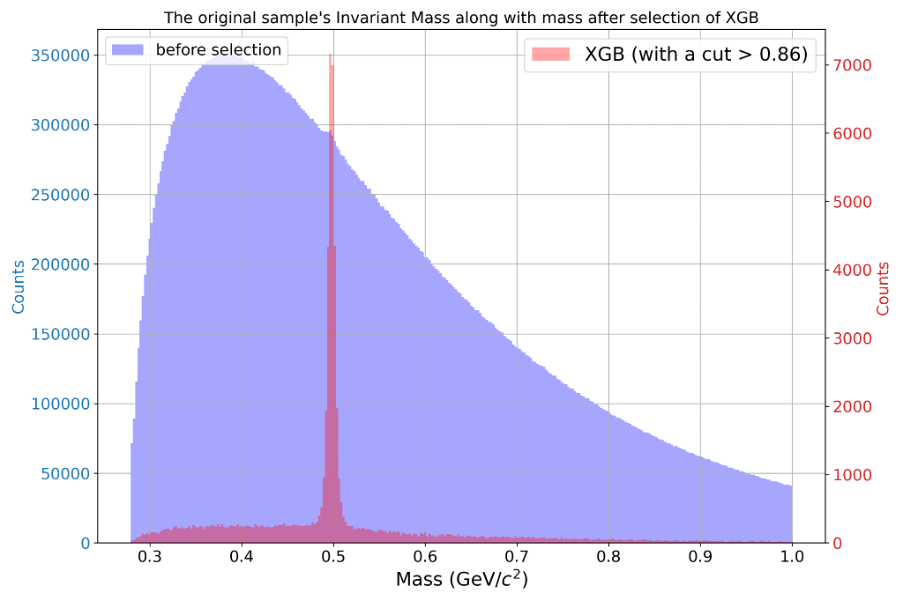
\includegraphics[width=\textwidth]{images/better_efficiency1.png} 
        \caption{Invariant mass distribution (y log scale)} 
        \vspace{0.3cm}
    \end{subfigure}
     \hfill
       \begin{subfigure}[b]{0.99\linewidth}
        \centering
        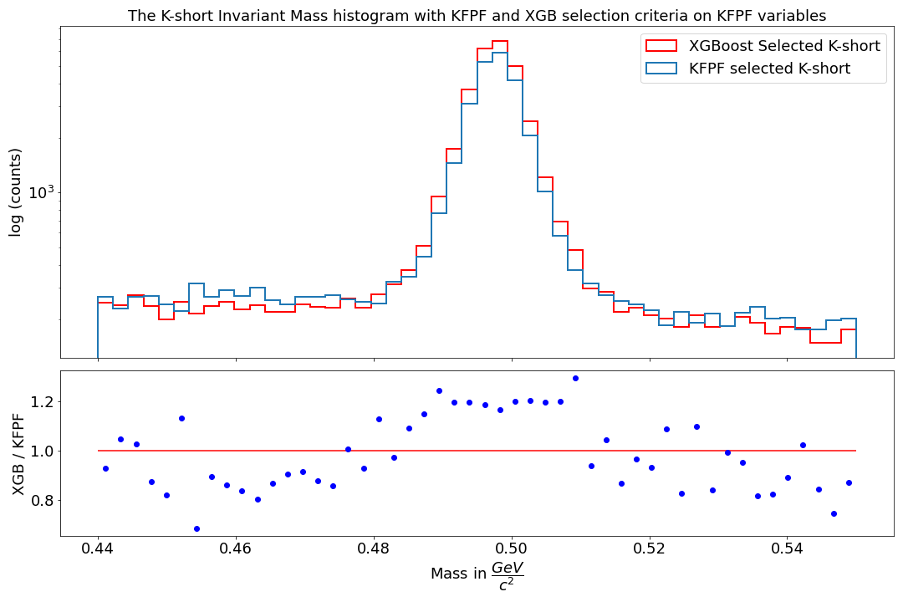
\includegraphics[width=\textwidth]{images/better_efficiency2.png} 
        \caption{Invariant mass distribution (close-up) - comparison with KFPF cuts}
        \vspace{0.3cm}
    \end{subfigure}
    \caption{Invariant mass distribution for probability $>$ 0.86}\label{effic}
\end{figure}

%--------------------- Investigation of potential bias
\subsection{Investigation of potential bias}
To check if the XGB selection criteria cut tails of the distribution, or are biased in some regions, the invariant mass distribution of true and false positives is plotted (Figure. \ref{true-false}).
\begin{figure}[h!]
 \centering
    \begin{subfigure}[b]{0.79\linewidth} 
        \centering
        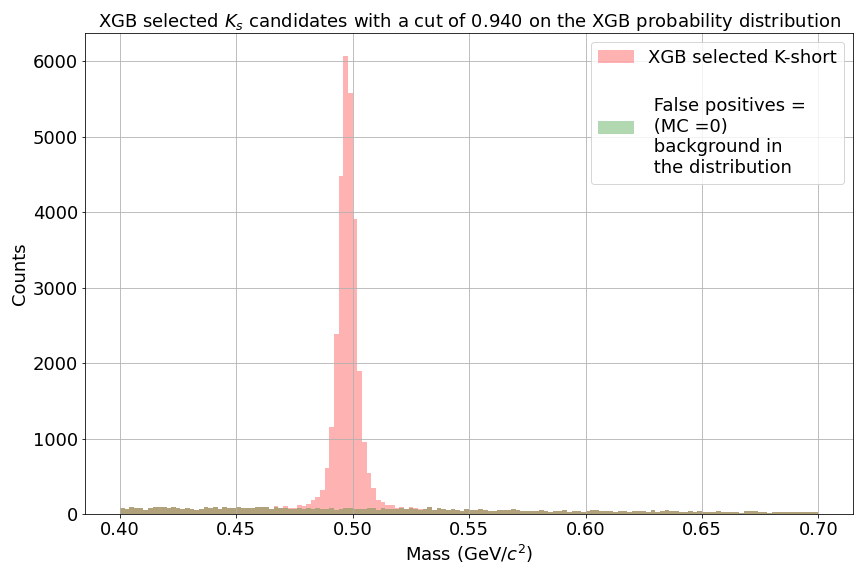
\includegraphics[width=\textwidth]{images/true_and_false_signal.png} 
        \caption{Selected \PKshort and false positives distribution} 
        \vspace{0.3cm}
    \end{subfigure}
     \hfill
       \begin{subfigure}[b]{0.69\linewidth}
        \centering
        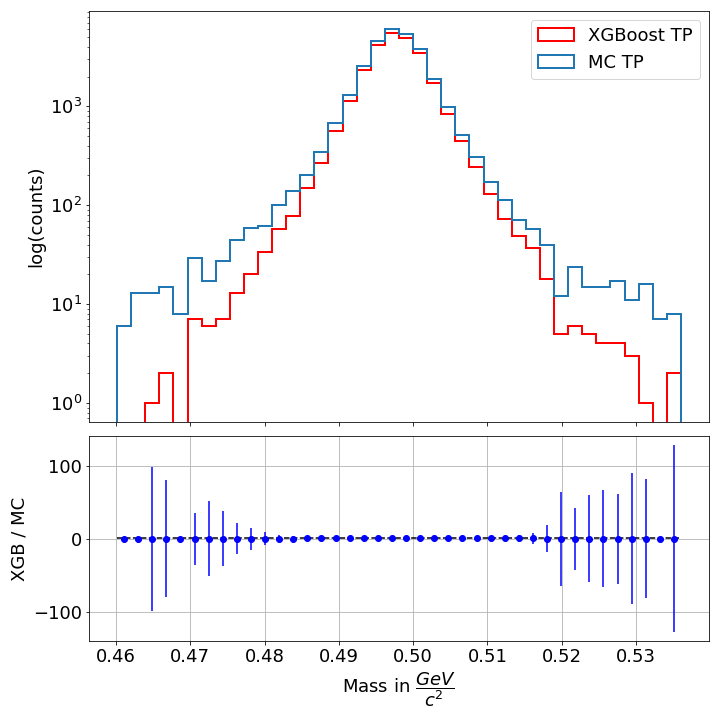
\includegraphics[width=\textwidth]{images/efficiency_plot_mass.png} 
        \caption{Reconstructed and MC true positives (y log scale)}
        \vspace{0.3cm}
    \end{subfigure}
    \caption{True-false positives investigation}
    \label{true-false}
\end{figure}
We see that our model does not seem to be biased towards any invariant mass region. Also, an investigation of influence of XGBoost on each variable has been performed.\cite{variables investigation}

\newpage
%----------------------- results for 3.3A GeV/c
\section{Results for $p_{\text{beam}}$ = 3.3A GeV/c}

\subsection{Comparison with KFPF cuts}
The same code can be used to obtain similar results for another CBM energy level. Comparing to default KFPF cuts, with probability cut 0.9635 (Fig. \ref{33agev}):
\begin{itemize}
    \item \textbf{Reconstructed \PKshort / reconstructible \PKshort = 93.45\%}  vs. 78.94\% with default KFPF cuts
    \item \textbf{false / true positive rate = 0.19} vs. 1.38 with default KFPF cuts
\end{itemize}

\begin{figure}[h!]
 \centering
    \begin{subfigure}[b]{0.99\linewidth} 
        \centering
        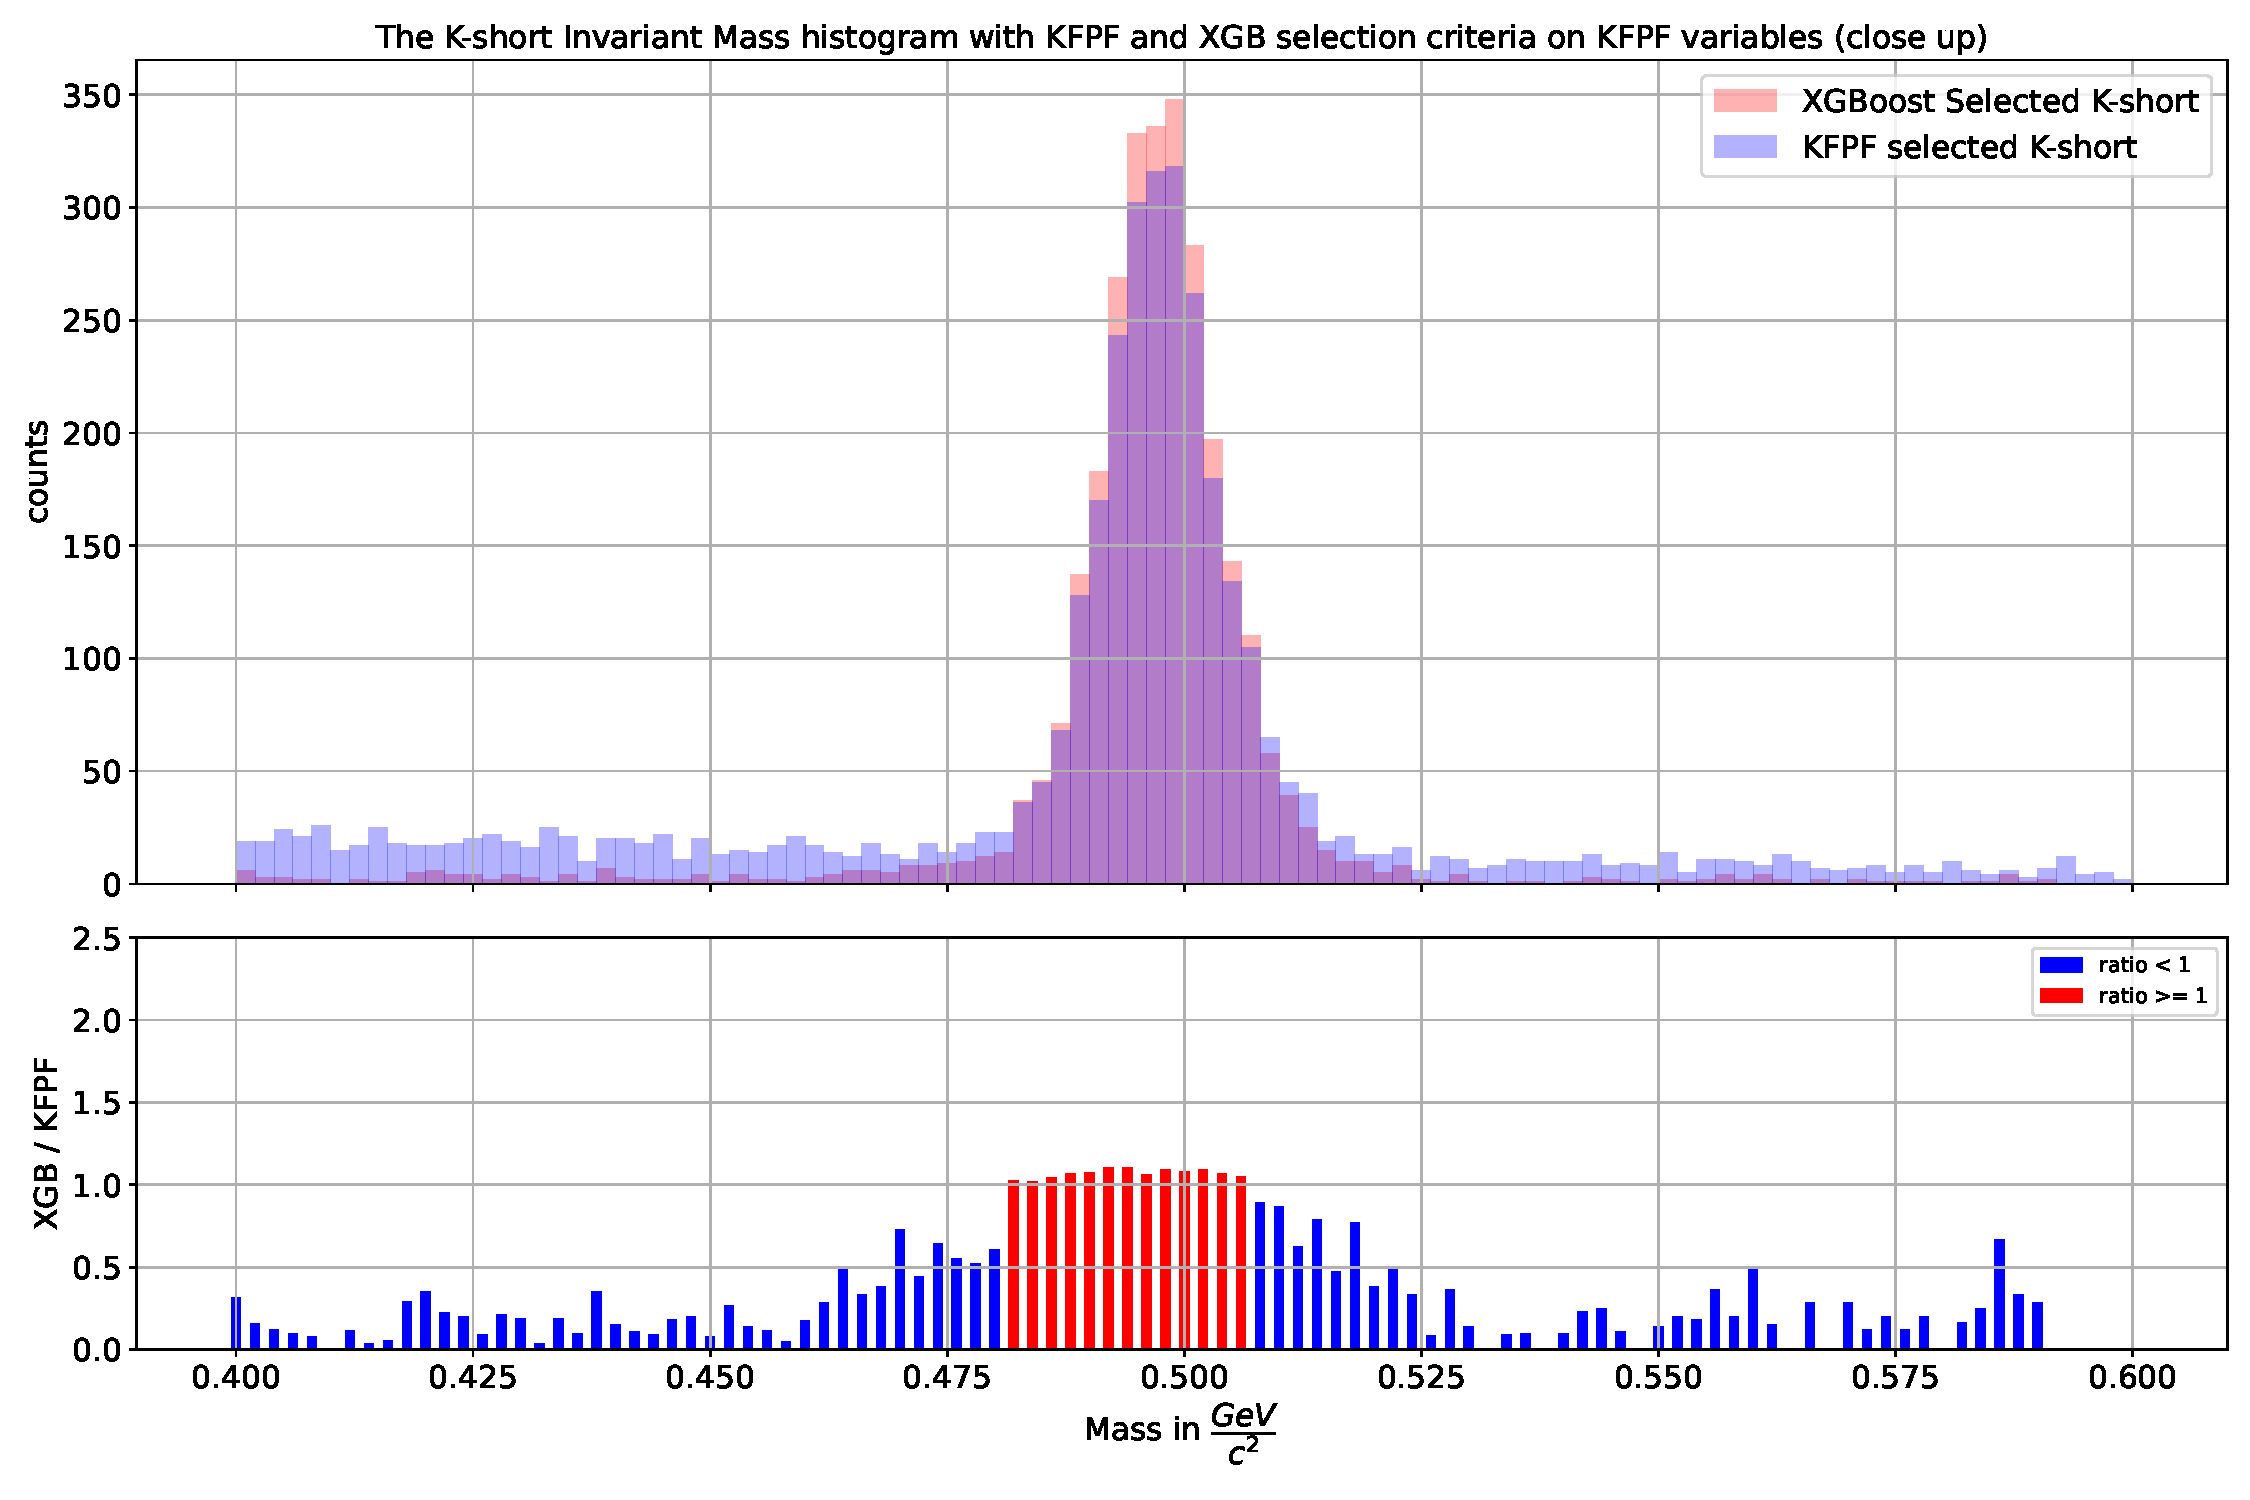
\includegraphics[width=\textwidth]{images/kaon_inv_mass_comparison_closeup.pdf} 
        \caption{Invariant mass distribution (y log scale)} 
        \vspace{0.3cm}
    \end{subfigure}
     \hfill
       \begin{subfigure}[b]{0.99\linewidth}
        \centering
        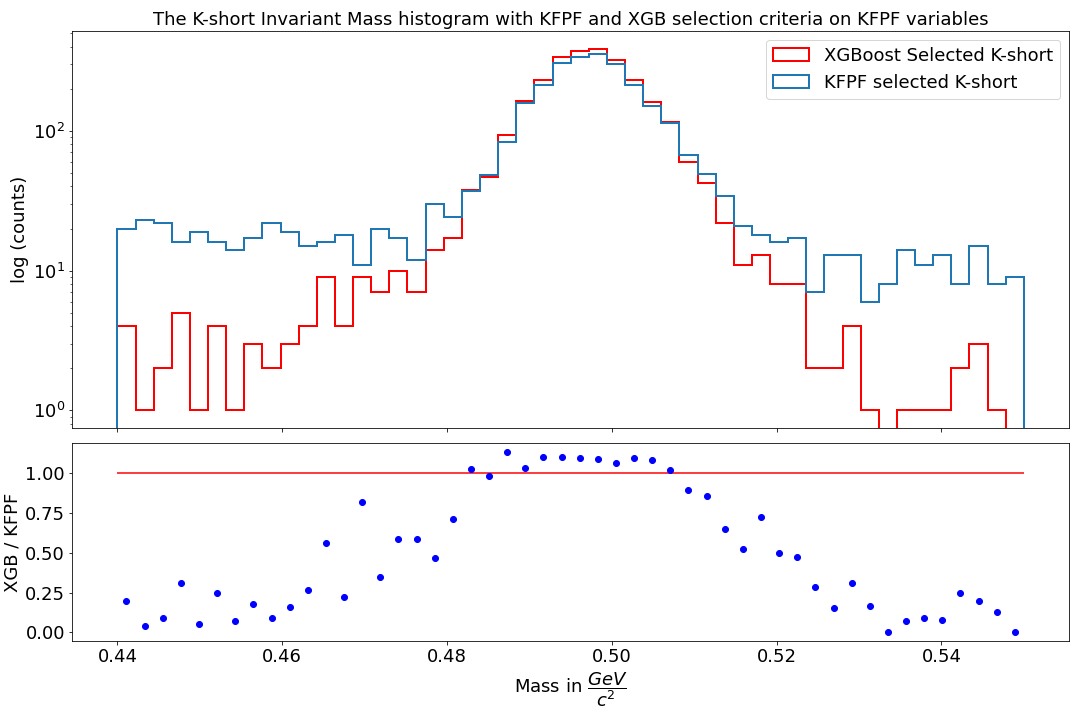
\includegraphics[width=\textwidth]{images/circle_kshort_invmass_with_ML.png} 
        \caption{Invariant mass distribution (close-up)}
        \vspace{0.3cm}
    \end{subfigure}
    \caption{Comparison with KFPF cuts for 3.3A GeV/c}\label{33agev}
\end{figure}
Due to the smaller statistics for this energy level, the ML model training should be redone for a bigger dataset.

%-------------- Influence of the magnetic field scaling
\subsection{Influence of the magnetic field scaling}
Obtained ML model can be adapted for the investigation of the influence of the magnetic field scaling. We compare: 100\% MF strength (for  $p_{\text{beam}}$ = 12A GeV/c), 56\% and 27.5\% MF strength (for $p_{\text{beam}}$ = 3.3A GeV/c, both with only DCM generated data for 0.4M events for training and 0.1M for validation). We see (Fig. \ref{mf}) that the stronger the magnetic field is, the broader \PKshort invariant mass distribution peak is. Also, we observe much more signal entries for $p_{\text{beam}}$ = 12A GeV/c (for the same number of events). \\

For $p_{\text{beam}}$ = 3.3A GeV/c the number of signal entries is almost the same; we select the probability cut so that the false/true positive ratio is the same for both \% of MF and compare the efficiency of the reconstruction (Tab. \ref{tab:mf}). We see that weaker MF does not necessarily worsen efficiency (only 2\% difference). However, this comparison should also be redone for a bigger dataset.

\begin{table}[h!]
\begin{tabular}{|l|l|l|l|}
\hline
\textbf{ratio} &
  \textbf{\begin{tabular}[c]{@{}l@{}}12 A GeV/c \\ MF=100\%\end{tabular}} &
  \textbf{\begin{tabular}[c]{@{}l@{}}3.3 A GeV/c \\ MF=56\%\end{tabular}} &
  \textbf{\begin{tabular}[c]{@{}l@{}}3.3 A GeV/c \\ MF=27.5\%\end{tabular}} \\ \hline
\begin{tabular}[c]{@{}l@{}}reconstructed/\\ reconstructible\end{tabular} &
  89.98\% &
  90.36\% &
  88.49\% \\ \hline
\begin{tabular}[c]{@{}l@{}}false / \\ true positive\end{tabular} &
  0.2 &
  0.2 &
  0.2 \\ \hline
\end{tabular}
\caption{\label{tab:mf}Comparison of MF strength vs. efficiency}
\end{table}

\begin{figure}[h!]
 \centering
    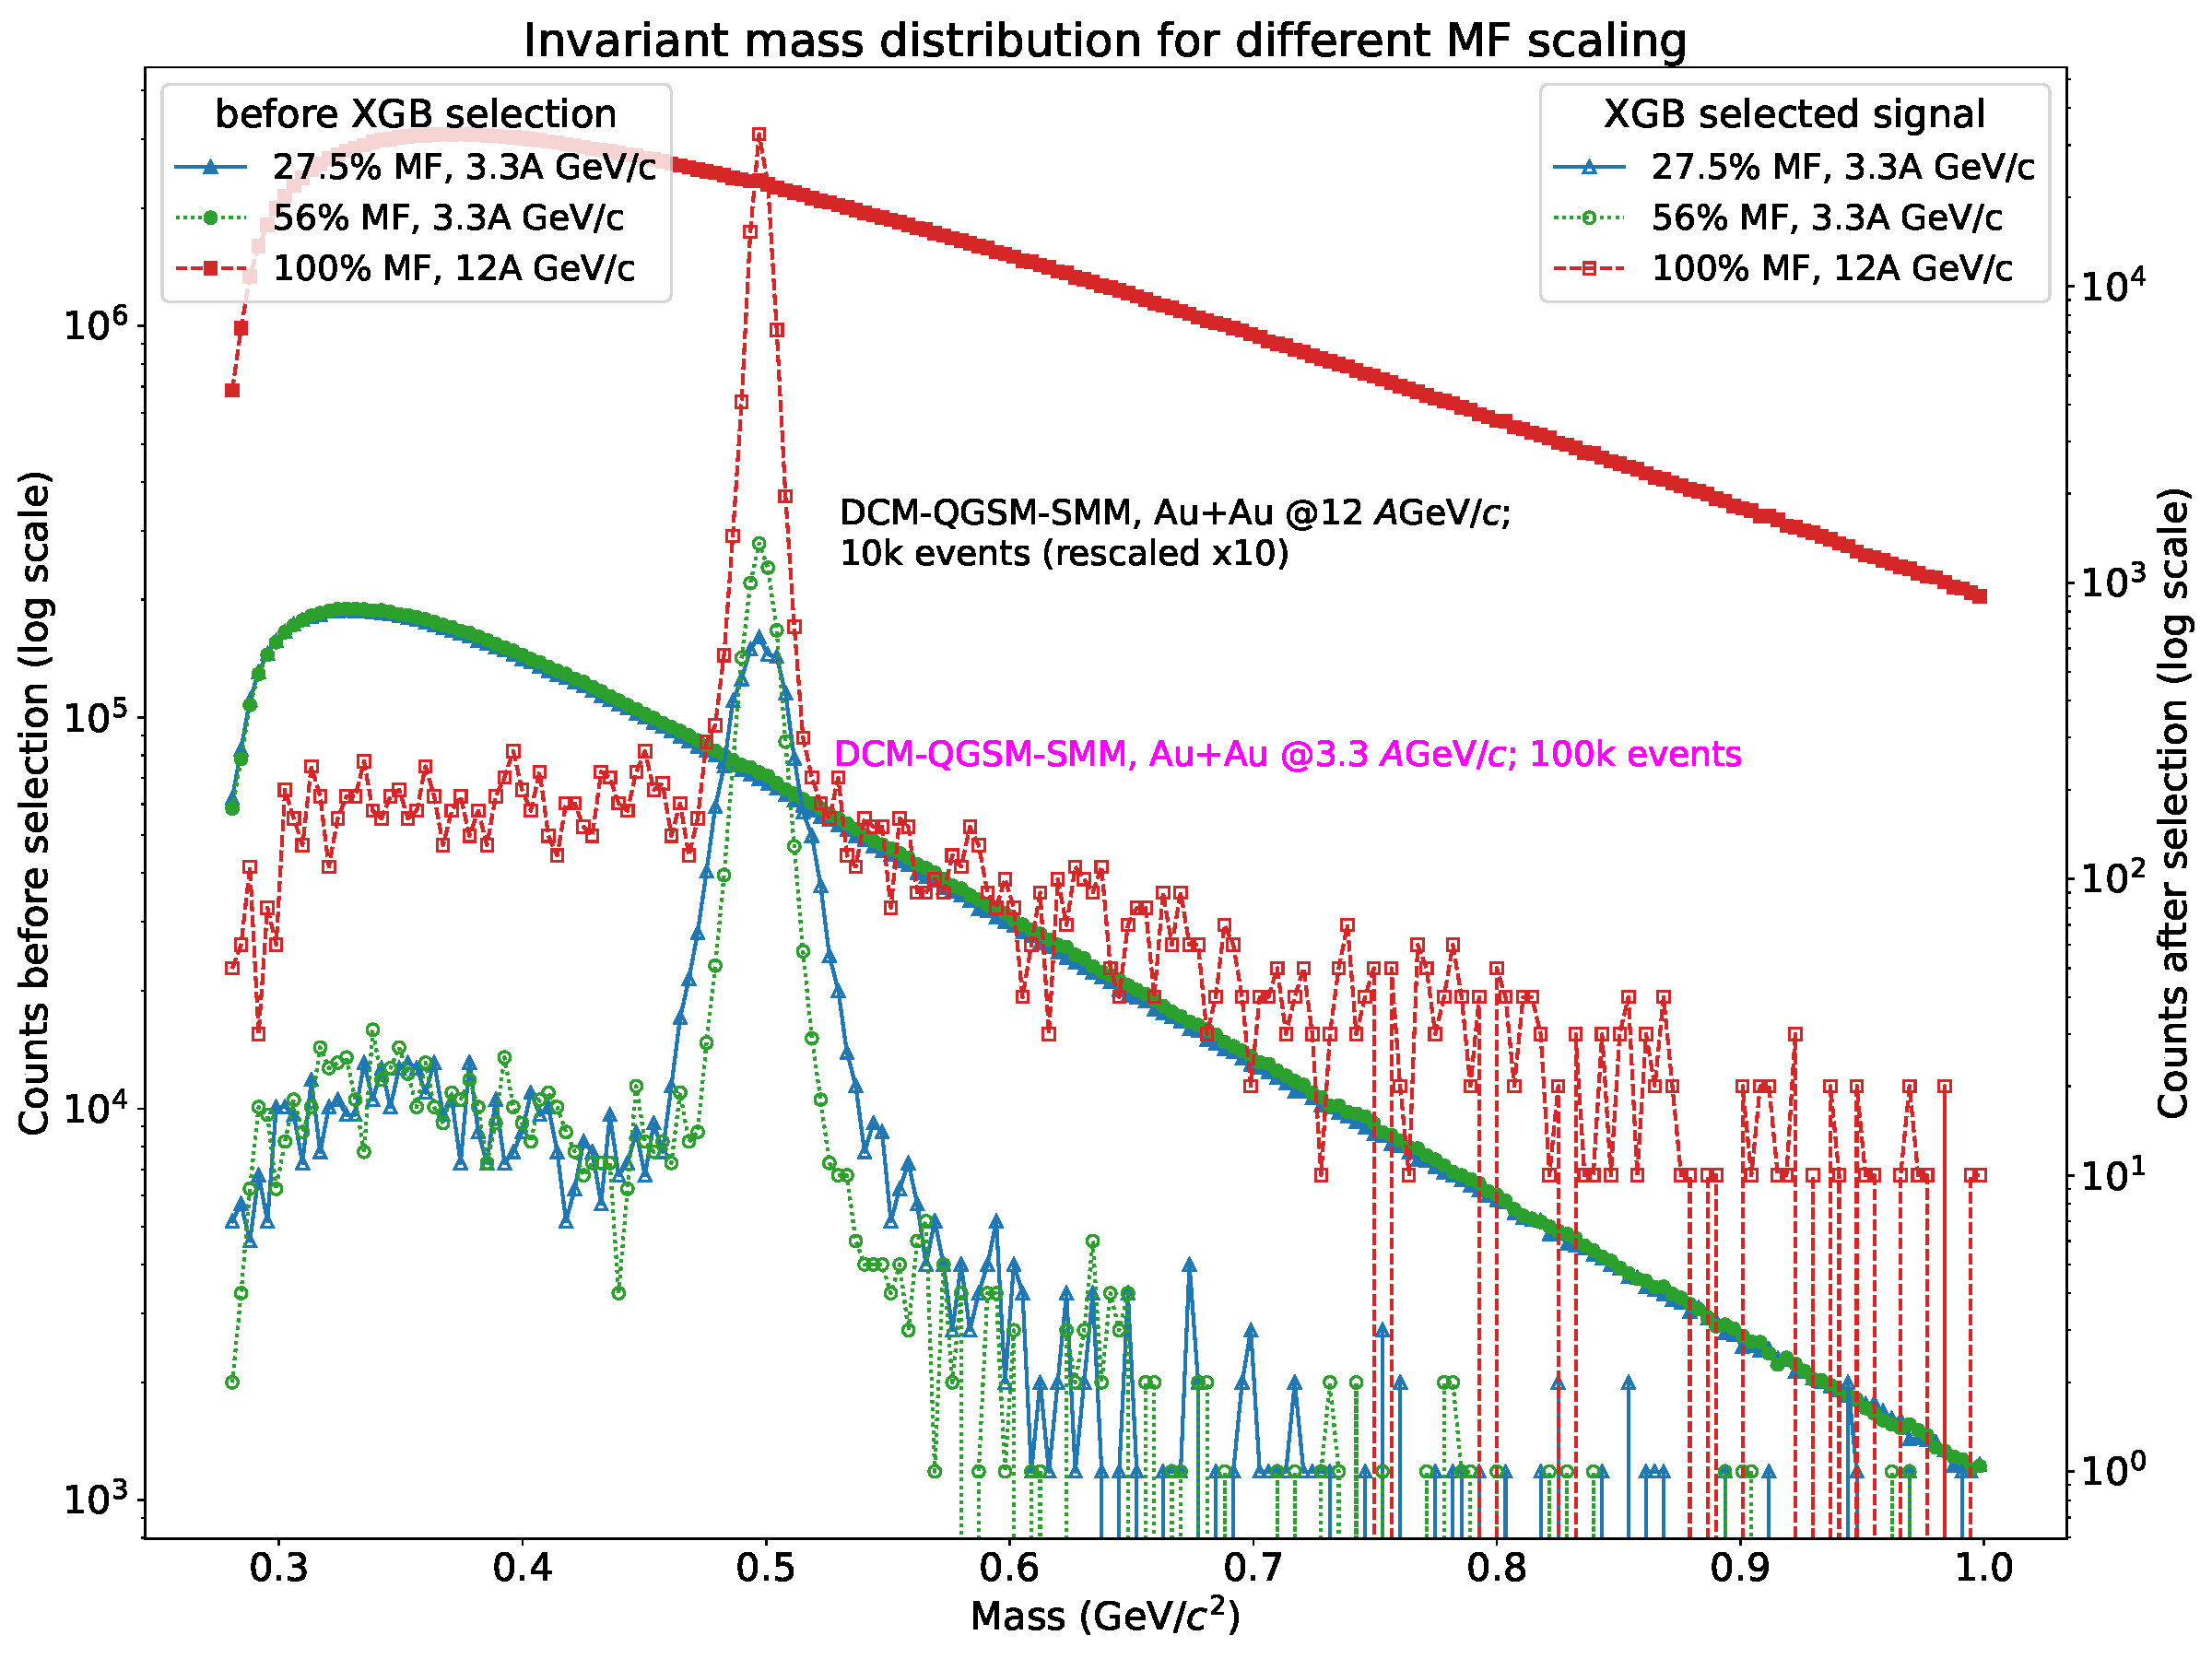
\includegraphics[width=\textwidth]{images/mf0log.pdf} 
    \vspace{0.1cm}
    \caption{Invariant mass distribution for different MF scaling}
    \label{mf}
\end{figure}

%------------------Summary and outlook
\chapter{Summary and outlook}
The optimization of \PKshort reconstruction at different collision energies ($p_{\text{beam}}$ = 12A GeV/c and 3.3A GeV/c) was performed. After preparing simulated data (enriching, cleaning, and variables selection) and loading them into XGBoost framework, we obtain a well working ML model which allows us to differentiate between the \emph{signal} - pion pairs created in K-short decay, and \emph{background} - pions pairs returned by KFParticle Finder, which are not the result of a \PKshort decay. We observe that a higher collision energy results in a bigger \PKshort production. Also, the investigation of influence of the magnetic field was performed - the efficiency of the reconstruction does not seem to be lower with a weaker MF; this investigation should be redone with a bigger dataset though.\\\\
Created framework can be applied to perform a multi-differential analysis of the selection optimization in transverse momentum, rapidity, and centrality at different collision energies. Also, the discriminator should be prepared to be imported to AnalysisTree in (Cbm)Root.



\chapter{Bibliography or References}
\begin{thebibliography}{9}

\bibitem{cbm-experiment} 
\url{https://fair-center.eu/for-users/experiments/cbm.html}

\bibitem{progress report}
"Compressed Baryonic Matter Experiment at FAIR, Progress Report 2020" Senger, Peter et. al (CBM Collaboration) doi:10.15120/GSI-2021-00421. 

\bibitem{prezentacja gosi}
\url{https://indico.gsi.de/event/13089/contributions/56358/attachments/37175/\\49720/38th\_CBM\_CollaborationMeeting\_KarabowiczMalgorzata\_MLforXi-Reconstruction.pdf}

\bibitem{tof}
M.~C.~S.~Williams,
``Particle identification using time of flight,''
J. Phys. G \textbf{39} (2012), 123001
doi:10.1088/0954-3899/39/12/123001

\bibitem{deconfinement}
M.~Orsaria, H.~Rodrigues, F.~Weber and G.~A.~Contrera,
``Quark deconfinement in high-mass neutron stars,''
Phys. Rev. C \textbf{89} (2014) no.1, 015806
doi:10.1103/PhysRevC.89.015806
[arXiv:1308.1657 [nucl-th]].

\bibitem{dcm}
M.~Baznat, A.~Botvina, G.~Musulmanbekov, V.~Toneev and V.~Zhezher,
``Monte-Carlo Generator of Heavy Ion Collisions DCM-SMM,''
Phys. Part. Nucl. Lett. \textbf{17} (2020) no.3, 303-324
doi:10.1134/S1547477120030024
[arXiv:1912.09277 [nucl-th]].

\bibitem{dcm2}
A.~S.~Botvina, I.~N.~Mishustin, M.~Begemann-Blaich, J.~Hubele, G.~Imme, I.~Iori, P.~Kreutz, G.~J.~Kunde, W.~D.~Kunze and V.~Lindenstruth, \textit{et al.}
``Multifragmentation of spectators in relativistic heavy ion reactions,''
Nucl. Phys. A \textbf{584} (1995), 737-756
doi:10.1016/0375-9474(94)00621-S
%157 citations counted in INSPIRE as of 04 Oct 2021

\bibitem{urqmd}
\url{https://urqmd.org/}

\bibitem{geant4}
S.~Agostinelli \textit{et al.} [GEANT4],
``GEANT4--a simulation toolkit,''
Nucl. Instrum. Meth. A \textbf{506} (2003), 250-303
doi:10.1016/S0168-9002(03)01368-8

\bibitem{geant4 2}
J.~Allison, K.~Amako, J.~Apostolakis, H.~Araujo, P.~A.~Dubois, M.~Asai, G.~Barrand, R.~Capra, S.~Chauvie and R.~Chytracek, \textit{et al.}
``Geant4 developments and applications,''
IEEE Trans. Nucl. Sci. \textbf{53} (2006), 270
doi:10.1109/TNS.2006.869826

\bibitem{kdecay1} 
\url{http://hyperphysics.phy-astr.gsu.edu/hbase/Particles/kaon.html}

\bibitem{kdecay2}
P.~A.~Zyla \textit{et al.} [Particle Data Group],
``Review of Particle Physics,''
PTEP \textbf{2020} (2020) no.8, 083C01
doi:10.1093/ptep/ptaa104

\bibitem{kfp}
\url{https://indico.cern.ch/event/773049/contributions/3476146/attachments/1939866\\/3218991/Kisel\_CBM\_CHEP-2019.pdf}

\bibitem{pfsimple}
\url{https://indico.gsi.de/event/10062/contributions/48045/attachments/33320/43053\\/PFSimple4Lambda\_Highlights\_36CM.pdf}

\bibitem{manual}
\url{https://indico.gsi.de/event/10126/contributions/362/attachments/229/363\\/PFsimple\_cuts\_MC-optimization.pdf}

\bibitem{ibm}
\url{https://www.ibm.com/cloud/learn/supervised-learning}

\bibitem{xgboost}
\url{https://xgboost.ai}

\bibitem{shahid}
S.~Khan, V.~Klochkov, O.~Lavoryk, O.~Lubynets, A.~I.~Khan, A.~Dubla and I.~Selyuzhenkov,
``Machine Learning Application for $\mathbf{\Lambda}$ Hyperon Reconstruction in CBM at FAIR,''
[arXiv:2109.02435 [physics.ins-det]].

\bibitem{non-linear}
\url{https://github.com/julnow/JupyterNotebooks/blob/kaon/img\\/correlations/bckgr\_mass\_pdf.pdf}

\bibitem{bayesian}
\url{https://github.com/fmfn/BayesianOptimization/}

\bibitem{variables investigation}
\url{https://github.com/julnow/JupyterNotebooks/blob/kaon/img\\/xgb\_12agev/chi2geo/params.pdf}


\end{thebibliography}

\end{document}